%!TEX root = ../main.tex

\chapter{Motif Annotation \& Classification}\label{ch:motif-classification}

\chapterprecishere{``A motif is the smallest element in a tale having a power to persist in tradition.''}{Stith Thompson}{The Folktale}

\section{Introduction}

In the introduction to his seminal \emph{Motif-Index of Folk Literature} (TMI), Stith Thompson addressed a number of fundamental challenges in folklore research. One crucial problem concerns ``the need for a comprehensive classification of the materials in all kinds of traditional narrative''\autocite[8]{thompson:1955}, which became all the more urgent in light of the ever-growing number of tales that were being collected at the time. Furthermore, he felt that the then current type index by Antti Aarne\autocite{aarne:1928} was not sufficient for indexing folktales from outside Europe. Thompson took it upon himself to try to remedy this situation by classifying folktales on the basis of motifs, which resulted in the first edition of the TMI in the 1930s\autocite{thompson:1932} and a revised and enlarged second edition in the 1950s that nearly doubled its scope\autocite{thompson:1955}.

In folktale research, motifs are a key concept in the classification of folktales into tale types. In the authoritative folktale type catalog, \emph{The Types of International Folktales}\autocite{uther:2004} -- a project initiated by Aarne in 1910 in his \emph{Verzeichnis der Märchentypen} (Catalogue of tale types)\autocite{aarne:1910}, which was translated and revised by Thompson\autocite{aarne:1928,aarne:1961} -- motifs form the primary descriptive units, and their configuration defines the folktale type of a story. There is, however, a large body of criticism aimed at the TMI as well as the different editions of the folktale type index, such as, for example, \citeauthor{dundes:1997} in relation to Aarne's 1961 edition\autocite{dundes:1997}, and \citeauthor{karsdorp:2012} with respect to Uther's most recent edition of the \emph{The Types of International Folktales}\autocite{karsdorp:2012}. This criticism has focused on the distribution and overlap of tale types and motifs. Furthermore, \citeauthor{el-shamy:1980} addresses the lacunae in the collection of sources used\autocite{el-shamy:1980}. Despite the various problems with respect to the applicability of the Aarne/Thompson folktale index to non-European tales, El-Shamy states that ``these can be adequately addressed through its [the folktale index's] relatively open classification system, which allows for adding new items, particularly when compared to other systems''\autocite[158]{el-shamy:1988}. Additionally, Alan Dundes states:
\begin{quote}
    It must be said at the outset that the six-volume \emph{Motif-Index of Folk-Literature} and the Aarne-Thompson tale type index constitute two of the most valuable tools in the professional folklorist's arsenal of aids for analysis. This is so regardless of any legitimate criticisms of these two remarkable indices, the use of which serves to distinguish scholarly studies of folk narrative from those carried out by a host of amateurs and dilettantes. The identification of folk narratives through motif and/or tale type numbers has become an international \emph{sine qua non} among bona fide folklorists.\autocite[195]{dundes:1997}
\end{quote}
While many new motif indices\autocite[See e.g.][]{baughman:1966,ideka:1971,kirtley:1977,childers:1977,flowers:1980,neuland:1981,el-shamy:1995} as well as many new collections of folktales\autocite{el-shamy:1980,meder:2000,slone:2001,crooke:2002} have since been put forward, relatively few attempts have been made to combine the two\autocites[Although see, in recent years][]{ben-amons:2006,slone:2001}[For further examples of both motif indices as well as folktale collections, see][]{uther:1996}. I hypothesize that the lack of combining the two resources is related to a lack of navigability of the TMI. Furthermore, while many of the researchers explicitly integrate their new indices into the TMI\autocite[For a brief and recent example, see][]{bell:2009}, there is no complete and combined edition of all these indices. Because of the problems that printing a book of such magnitude would generate, it is understandable that such an edition is unavailable. These considerations would evaporate for a digital edition. Yet, however valuable a research tool it would be, no digital edition exists at present. Given the TMI's unquestioned status as \emph{the} source for the worldwide coverage of folk narrative, a search engine of the TMI would be of interest to many scholars, ranging from folklorists to narratologists and story generation researchers.

The aims of the present chapter are the following. First, I wish to highlight some of the navigational challenges one has to overcome in order to make use of existing motif indices successfully, taking the TMI as a case study. I agree with Harriet Goldberg that ``[t]he utility of an index of folk-motifs clearly lies in its ability to present in an orderly framework those transitory flashes of recognition that we experience upon hearing a familiar story or a familiar narrative component in a new context''\autocite[xiii]{goldberg:1998}. To meet this objective, I present \emph{Meertens Online Motif FindER} (MOMFER), which is a free, online search engine designed to increase the accessibility of the TMI.\footnote{Available at \url{http://www.momfer.ml}} This tool provides various new and unique access points to the index, drawing inspiration from techniques used in the fields of Natural Language Processing and Information Retrieval.\autocite[For a similar approach that attempts to enrich the motif index with semantic information, cf.][]{declerck:2011} MOMFER enables several different search options: besides basic options such as single word, multi-word, and phrase searches, it is also possible to use faceted search, and even semantic search. These options, I suggest, can provide new tools for researchers and can lead to the asking and answering of questions that were hitherto deemed unanswerable. Furthermore, there is great potential for this tool to be used as a framework into which all other existing motif indices will be integrated.

Second, one is confronted with the problem that, although the motif search engine MOMFER provides researchers with a indispensable research tool to more efficiently access and retrieve information from the TMI, it remains rather cumbersome and time-consuming to manually label folktales with their corresponding motifs. This is especially the case in large-scale collections such as the Dutch Folktale Database.\autocite{meder:2010,meder:2016} In order to reduce the amount of manual labor, then, I will develop a computational system with which motifs can be automatically assigned to folktales. If this automated motif classification system is combined with MOMFER, the analysis of large-scale folktale collections is greatly facilitated, which will aid and enhance future research aimed at mapping out relations between stories and their motifs.

The present chapter is structured as follows: first, I will briefly introduce the TMI to those readers who may be unfamiliar with it, which is followed by a discussion of some important navigational challenges associated with its use (Section \ref{sec:momfer-accessibility}). Subsequently, I will describe the creation process and architecture of MOMFER (Section \ref{sec:momfer-production}), after which I will proceed to highlight a number of interesting search options by presenting several case studies that use the TMI as a corpus (Section \ref{sec:momfer-case-studies}). The second part of this chapter is devoted to the development of the automated system for motif identification (Section \ref{sec:motif-classification}). 

\section{MOMFER}

\subsection{Accessibility of the \emph{Motif-Index}}\label{sec:momfer-accessibility}

The TMI\autocite{thompson:1955} contains over forty-five thousand motifs spread out over five volumes. The motifs are hierarchically ordered in a tree structure. There are twenty-three top-level, alphabetically labeled categories, whose contents range from mythological motifs (Category A) to motifs concerning traits of character (Category W) and beyond. Each top-level category is divided into various subcategories: for example, Category D (\emph{Magic}) is divided into, inter alia, \emph{Transformation} (D0--D699) and \emph{Magic Objects} (D800--D1699), which in turn branch out into child motifs, and so on and so forth. At the leaves of the tree, or terminal nodes, we find the most specific instances of a particular motif\autocites[For an elaboration on the build-up of the index and search strategies, see][Volume 1, 19–25]{thompson:1955}[16--17]{el-shamy:1995}. Figure \ref{fig:thompson-tree} is an exemplary representation of part of the hierarchical tree.

\begin{figure}
    \centering
    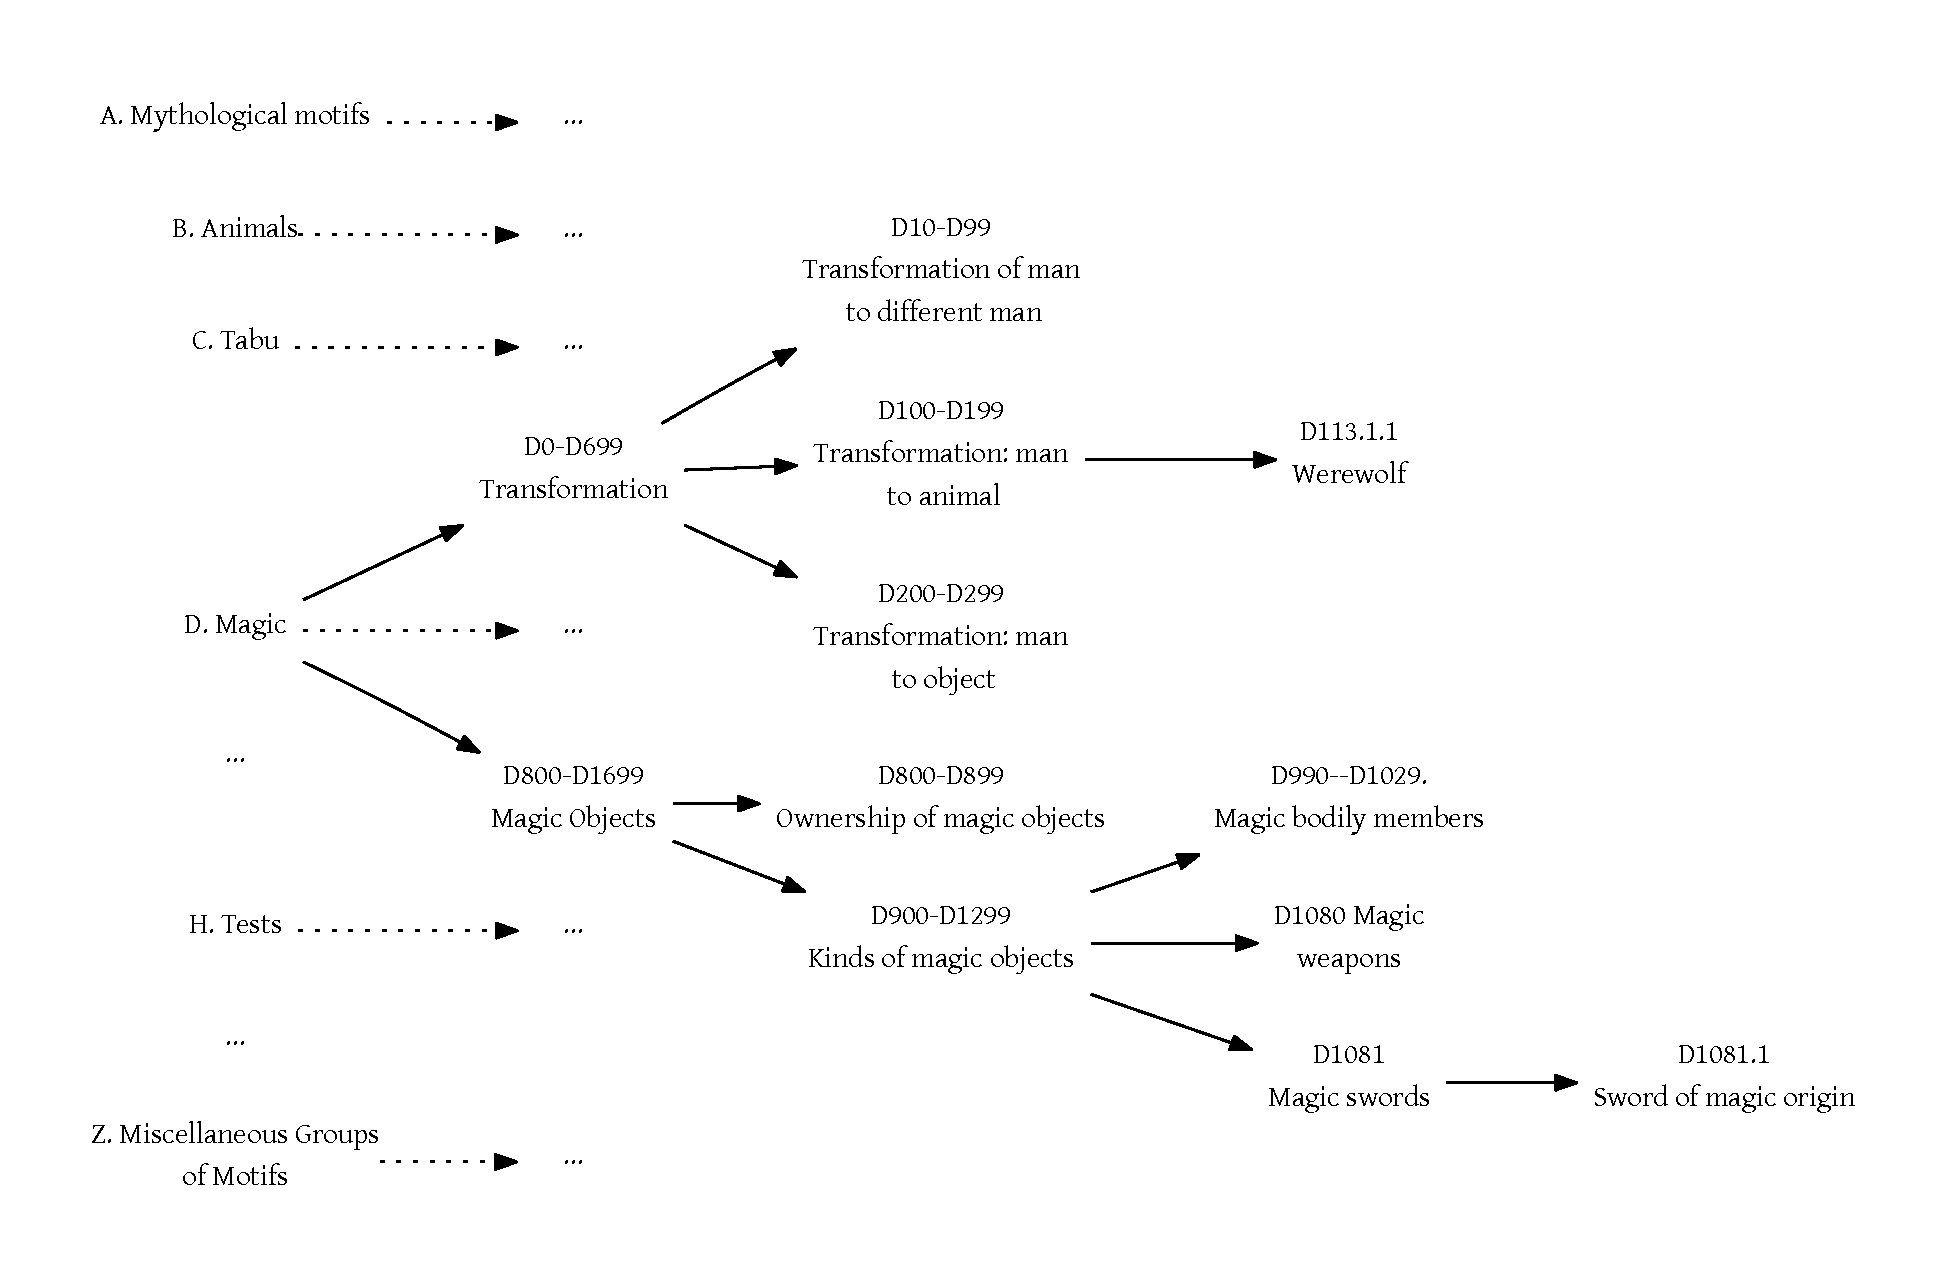
\includegraphics[width=\textwidth]{images/thompson-tree.pdf}
    \caption{Partial view of Thompson's \emph{Motif-Index of Folk Literature}.}
    \label{fig:thompson-tree}
\end{figure}

As Thompson states himself, the motifs in the first five volumes are grouped together as the result ``of a gradual evolution, not of any preconceived plan''\autocite[19]{thompson:1955}. This method (or lack thereof) has several potential negative effects. First, as can be seen from Figure \ref{fig:tmi-motif-distribution}, the distribution of the motifs over the main categories in the index is rather uneven, with categories A -- K containing seventy-eight per cent of all motifs in the index. Second, the index lists seventy-two motifs twice under different headwords (i.e.\ 144 unique motifs). For example, the motif \emph{Transformation: utensil to person} has been indexed both as D436.1 and D434.1. Other examples include \emph{One day and one night: object borrowed for a day and a night retained} indexed under K2314.1 and K232.2, and \emph{Well shines at night}, which is categorized at two completely separate branches of the tree: \emph{Magic} (D1645.9) and \emph{Marvels} (F718.5). These cases represent the extreme endpoint on the scale of a more general problem that, as observed by Dundes, many motifs from different branches show a high degree of semantic similarity.\autocite{dundes:1997}

\begin{figure}[t]
    \centering
    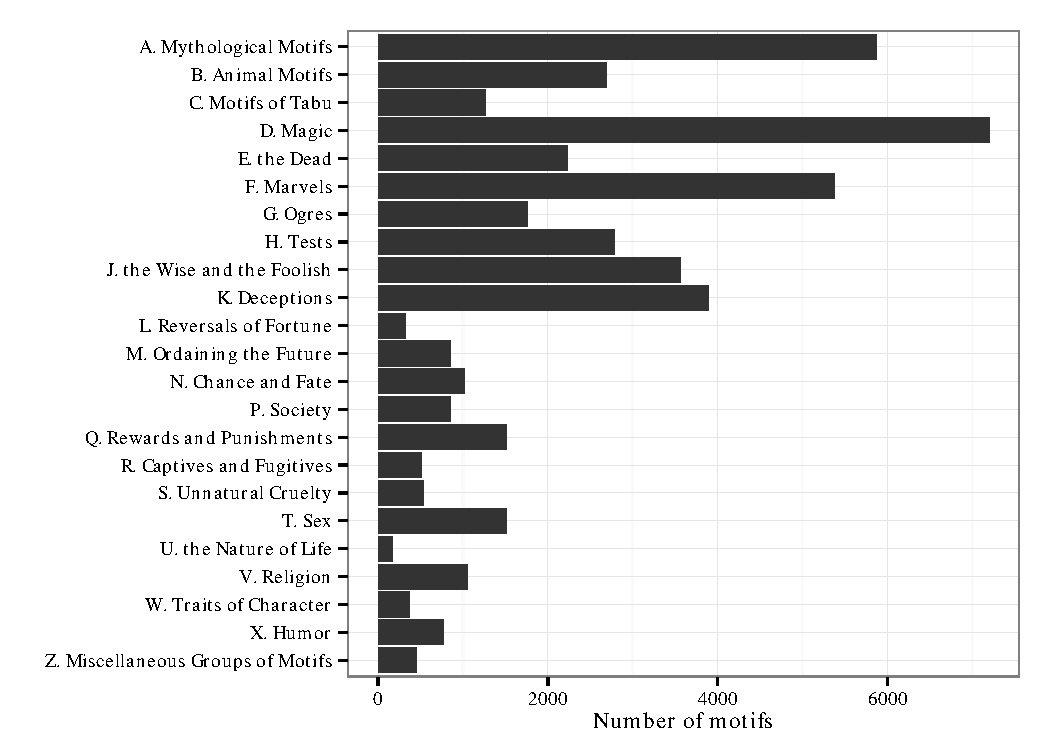
\includegraphics[width=\textwidth]{images/tmi-motif-distribution.pdf}
    \caption{Distribution of motifs over main branches of the \emph{Motif-Index of Folk Literature}.}
    \label{fig:tmi-motif-distribution}
\end{figure}

Volume Six of the TMI consists of an alphabetical index to the other five volumes. This index provides a different entrance point to the motif index using an alphabetically sorted list of important terms that appear in the other five volumes. Looking under the term \emph{mice}, for example, we find motifs such as the following (where the headword is left out):
\begin{itemize}
    \item~[mice] army saves kingdom from invasion K632.1;
    \item~[mice] consecrate bishop (lie) X1226.1;
    \item~[mice] and hogs let loose put elephant cavalry to flight K2351.3.
\end{itemize}
The examples are ordered on different levels. The first level is an alphabetical ordering of the second word of the motif, where the headword is the first word. For instance, as the example above shows, a motif starting with \emph{army} comes before one starting with \emph{consecrate}. However, as can be seen in the same example, this structure is not completely consistent: Thompson ignored function words such as \emph{and}, \emph{with}, and \emph{of}, so that after \emph{consecrate} comes \emph{and hogs}.

After this first set of motifs, a second set of motifs is listed that do not start with the
headword but do contain it:
\begin{itemize}
    \item army of m. B268.6;
    \item bargain with king of m. M244.1.
\end{itemize}
While this approach may at first glance seem quite unproblematic, it soon becomes troublesome when entries have a larger number of associated motifs. For example, the word \emph{horse} has over five pages with motifs listed (including \emph{horse's} and \emph{horses}). Here it quickly becomes cumbersome to read through all the motifs in the hopes of finding the appropriate one. Also, several stratagems have been undertaken by Thompson to save space: these include referring readers to a certain category (as for headword \emph{devil}: ``*G303ff.\ See, in addition to the following, the extensive list of motifs assembled at G303'') and listing certain sets of motifs together without details pertaining to the content of the motifs (as for headword \emph{cat}: ``and witches D1766.4, G211.1.7, G224.11.12, G241.1.4, G225.3, G243.2.2, *G252, G262.1.1, G262.3.2''). Thompson left room for new motifs -- although his reasons for doing so were in some cases, such as the erotic and scatological dimensions, suspect\autocite{legman:1962} -- and this room has been gratefully filled up by subsequent scholars. New motif indices are made compatible with the TMI by integrating newfound motifs into the hierarchical structure of the TMI. For example, Ernest W. Baughman\autocite{baughman:1966} posits the motif \emph{Transformation: man meets and copulates with female snake} as D191.2, as an addition to Thompson's D191: \emph{Transformation: man to serpent (snake)}. While this shows that a complete motif index is (at least theoretically) possible, the compilation of such an index far exceeds printing possibilities. Even Thompson himself was aware of this, and left out certain parts of folklore because ``To have included these would have doubled the size of the index''\autocite[11]{thompson:1955}, and an online version integrating all subsequent motif indices has as yet not been undertaken. Nevertheless, such a complete work is something to be desired, as it would provide a more comprehensive starting point for comparing different narrative traditions, which was, ultimately, the goal of the TMI\autocite[9--10]{thompson:1955}.

Today, with most of our digital search results only a few clicks away, the time-consuming labor of manually searching through the TMI, hoping to stumble upon the entry we are looking for, appears rather outdated. In response to this, several initiatives have been undertaken to make a version of the TMI available in digital format, both offline and online.\footnote{For an online example, see \url{http://www.ruthenia.ru/folklore/thompson/}.} The first example of this kind, as far as I am aware, is the CD-ROM edition of the TMI as published by Indiana University Press in 1993\autocite{thompson:1993}. While this version allows users to enjoy some of the benefits of digital searches (e.g.\ `Boolean searches'), it is not readily available, and it is safe to say that it is outdated, since its system requirements are ``DOS 2.0 or higher''\autocite[Unfortunately, I was unable to acquire a copy of this edition, which is why I have to refrain from a more detailed comparison. However, the fact that no research institution or university library in the Netherlands has a copy available is a case in point. I base myself on a review of this digital edition by][]{smith:1994}. By presenting the TMI in a digital format, users are able to search through the index using the search facilities provided by their web browser (such as the omnipresent `Find' function). Although this seems to be quite an improvement over searching through the paper index, in reality the improvements are small: queries remain limited to single expressions and/or phrases. There is one online search engine available at \url{www.storysearch.symbolicstudies.org}. Unfortunately, this search engine is limited in its applications: searches seem to be confined to one word, and documentation on other options is unavailable. Also, it does not seem to be intended as a search tool, more as a source of inspiration for storytellers. In conclusion, the benefits of the currently available digital and online versions are rather small in comparison with the paper version.

\subsection{Meertens Online Motif FindER (MOMFER)}\label{sec:momfer-production}

In this section I will introduce MOMFER. First, I will describe the architecture of the search tool, including the sources used and some of the preprocessing steps that were performed. Subsequently, I continue with an in-depth description of the most salient search features implemented in the tool. Figure \ref{fig:momfer} is a representation of the web interface of MOMFER.

\begin{figure}
    \centering
    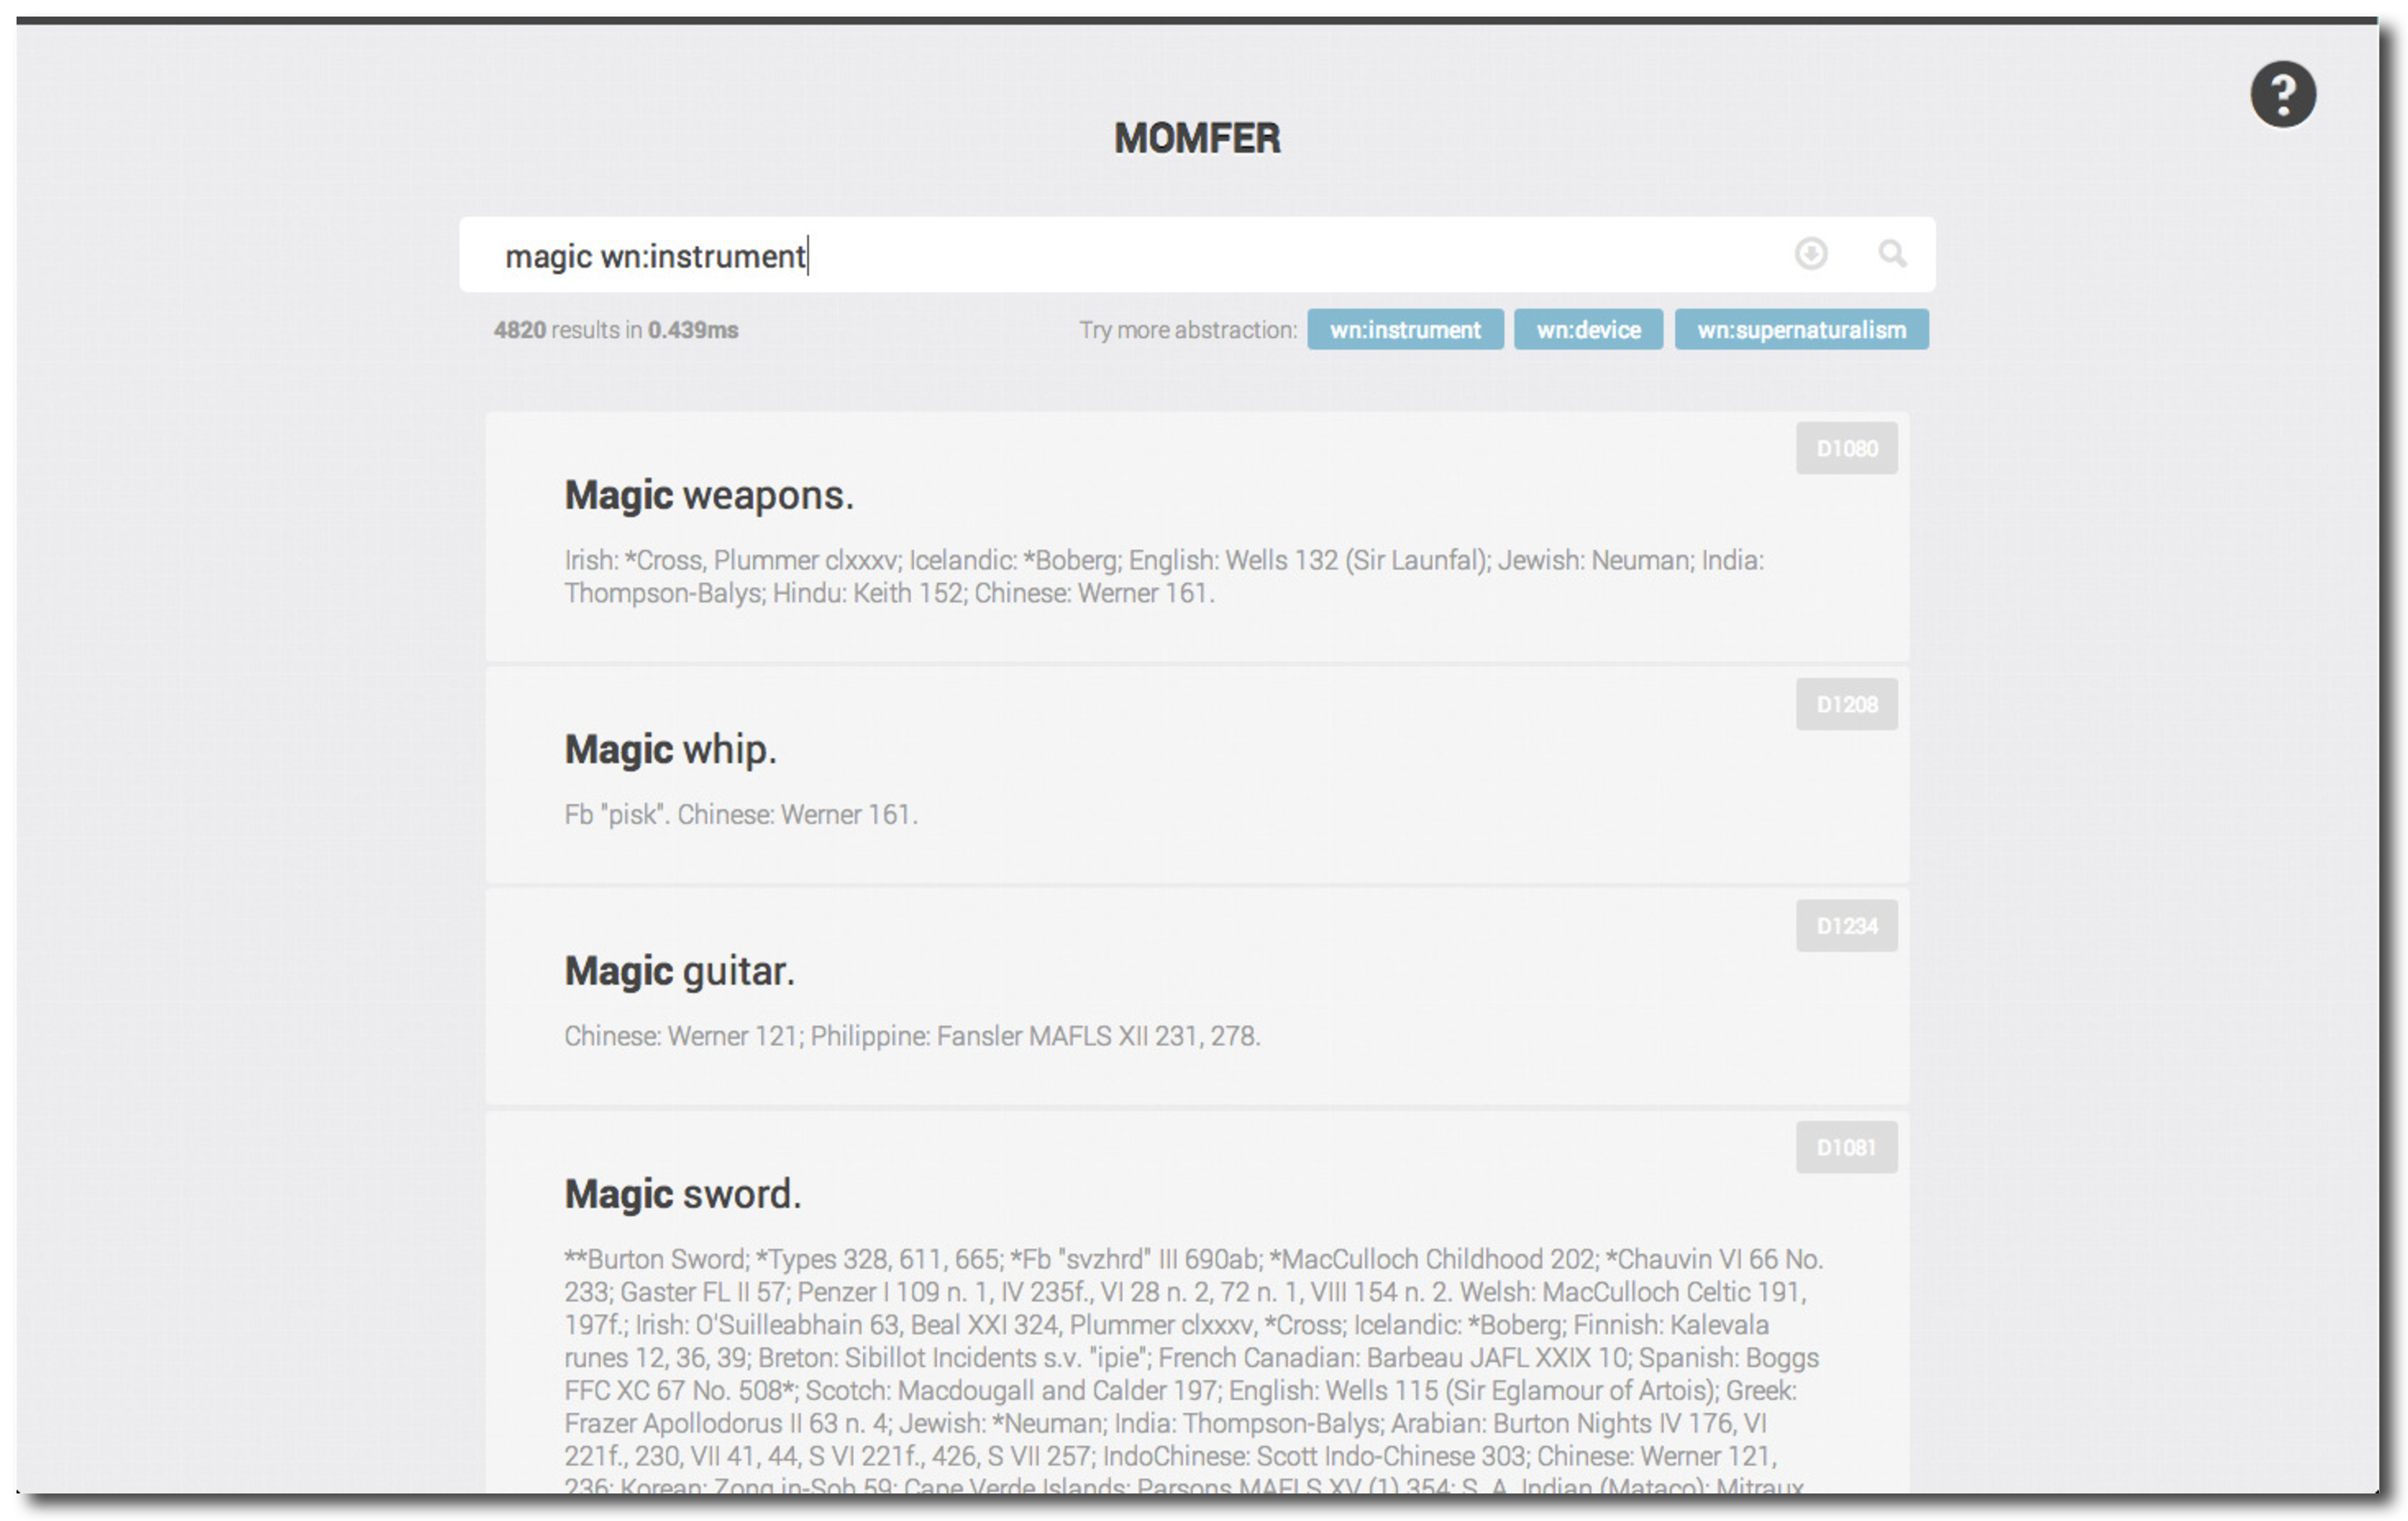
\includegraphics[width=\textwidth]{images/momfer.pdf}
    \caption{Web interface of the Meertens Online Motif FindER.}
\label{fig:momfer}
\end{figure}

\subsubsection{Preprocessing Steps}
As mentioned above, there are a few digitized versions of the TMI in existence. For this study, I constructed a full-text version of the motif index using the edition made available online at \url{http://www.ruthenia.ru/folklore/thompson/}. This digital edition is based on the revised and enlarged edition of the TMI\autocite{thompson:1955}. This edition was subjected to a number of preprocessing steps, which will be described in order. After stripping all of the HTML tags from the digital index, the `Stanford CoreNLP toolkit' (version 3.3.1)\autocite{toutanova:2003} was employed to tokenize all motifs into formally bounded sentences. The same toolkit was used to lemmatize and tag all words by part of speech (e.g.\ nouns, verbs, etc.) and to apply named entity recognition.

Although earlier writers have classified the motifs in the TMI as having a tripartite structure\autocite[Notably][]{el-shamy:1995}, for the purposes of this study I interpret each motif in the TMI as consisting of four parts: (i) a unique key, denoting the place in the hierarchy (consisting of a upper-level letter and a lower-level number key), (ii) a primary description, (iii) a secondary description (which is optional), and (iv) bibliographical information. After preprocessing a motif string such as ``C662. One must eat ``death vegetable'' whenever one sees it. Otherwise god will be angry. India: Thompson-Balys.'', it is represented in JSON format as follows:

\begin{verbatim}
{
  "motif": "C662", 
  "description": "One must eat \"death vegetable\" whenever 
                  one sees it.", 
  "lemmas": [
    "vegetable", 
    "death"
  ], 
  "locations": [
    "India"
  ], 
  "additional_description": "Otherwise god will be angry.", 
  "references": "India: Thompson-Balys."
}
\end{verbatim}

\noindent Here \texttt{motif} represents the unique key as given by Thompson; \texttt{description} and \texttt{additional\_description} provide a verbal characterization of the motif, where the second part is usually an explication of the first part; \texttt{references} points to any references and bibliographic information (e.g.\ collector, collection, and/or location) available for this motif; \texttt{lemmas} stores the lemmatized versions of nouns in the description field; \texttt{locations} lists all mentions of geographical locations in the reference field. With the help of a number of programming scripts, I extracted these fields for all motifs in the index.\footnote{The parsed index as well as the source code of MOMFER is available online at \url{https://github.com/fbkarsdorp/tmi}.}

\subsubsection{Semantic Expansion}

One of the key features of our search engine is the way in which motifs are semantically expanded to match more generic descriptions. If a user issues a query such as \texttt{color animal}, the system should not only return `direct hits' (motifs in which both words occur), but also motifs containing instances of these words with either a higher or a lower specificity, such as B731.2 \emph{Green horse}. In order to do so, all lemmatized nouns and adjectives in the motif descriptions were matched against the semantic lexicon WordNet\autocite{fellbaum:2005}. WordNet is a large semantic lexicon of English, in which words of various syntactic categories are grouped into sets of related words, or `synsets'.\autocite[While there has been some criticism of the usefulness and limitations of WordNet, our case studies show that, for the purposes of this research tool, synsets and WordNet are in fact valuable methods that improve the retrieval results, cf.][]{wilks:1996,lenat:1995} The relations between different synsets are encoded by means of super-subordinate relations (or hyperonyms). Thus, a word like \emph{furniture} is linked to both more specific examples (or hyponyms) such as \emph{bed} and \emph{chair} and more general concepts (or hyperonyms) such as \emph{artefact}, and ultimately \emph{entity}, which forms the root node of the network (cf.\ Figure \ref{fig:wordnet-example}). While it is possible to search for such far-removed parents, MOMFER by default returns only the two immediate parental relations, primarily for efficiency reasons and also because a complete expansion would return all motifs in every query, only in different orderings.

\begin{figure}
    \centering
    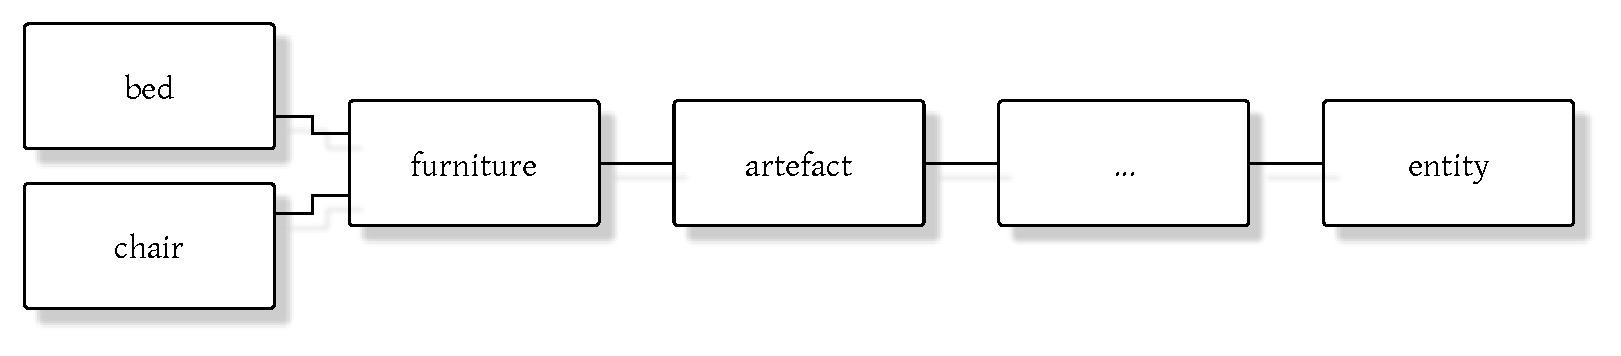
\includegraphics[width=\textwidth]{images/wordnet-example.pdf}
    \caption{Example of hyperonymic and hyponymic relations in WordNet.}
    \label{fig:wordnet-example}
\end{figure}

By linking motifs with words in other motifs on the basis of hyperonymic relations, the search engine provides a completely new way of accessing the TMI. This enables one to find many related motifs that are otherwise difficult to detect. To give a small example, say we are interested in the various occultists present in the TMI. The umbrella term \emph{occultist} does not occur at all in the index, yet we know the index is packed with motifs about witches, wizards, sorcerers, druids, magicians, enchanters, and so forth. In WordNet all these words are connected through the hyperonym \emph{occultist}. By connecting motifs based on their hyperonymic relations with other motifs, the system allows users to extract all types of occultists using the single search query \texttt{occultist}.\footnote{When linking the words from the TMI to the entries in WordNet, I did not perform any semantic disambiguation. Each word was linked to the most common sense in WordNet. In a later stage, this heuristic could be further refined.}

\subsubsection{Indexing Schema}

Figure \ref{fig:index-schema} provides a detailed view of the indexing schema. All motifs are preprocessed and fed to an indexer. This indexer extracts the various fields described above and stores the result in an index. When a user issues a search query, the index retrieves the top results which, after scoring and sorting, are presented to the user.\footnote{I make use of the programming library \emph{Whoosh}, which is a fast Python-based search engine library. See \url{http:// whoosh.readthedocs.org/}.}

\begin{figure}
\centering
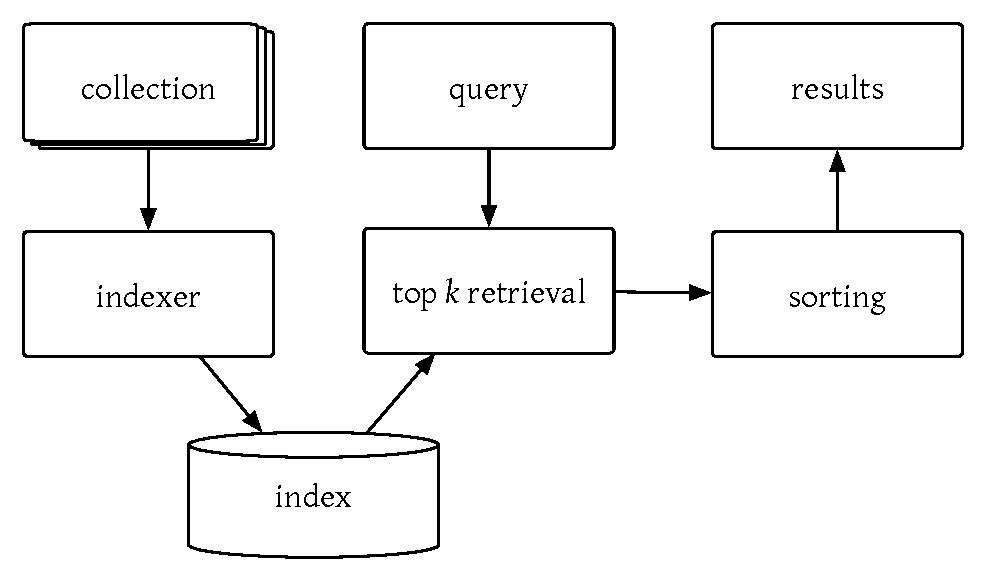
\includegraphics[width=\textwidth]{images/index-schema.pdf}
\caption{MOMFER's Search engine schema.}
\label{fig:index-schema}
\end{figure}

The system assumes that not all matches are equally important. If, for example, a user enters the query \texttt{book}, motifs that contain the word \emph{book} in the reference field are intuitively less relevant than those in which it is part of the primary description. To reflect this intuition, the system weighs the matches in the different fields in the following descending order: (i) primary description, (ii) additional information, (iii) WordNet expansion, and (iv) bibliographical information and location (references). Thus, a query for the word \emph{book} will first return motifs where the word is found in the primary description and/or additional information, before it turns to motifs matching the WordNet expansion.

\subsubsection{Query System}

MOMFER provides an expressive and rich query system, allowing users to retrieve their results efficiently. In this section I will describe the most important search features implemented in the tool.

Single word search is the simplest form of search, where users search for a single word. The index retrieves all motifs containing the search word and ranks them according to how informative the word is for that particular motif. If, for example, a user searches for the word \emph{devil}, the motif G303 (`Devil') will be ranked highest because it contains no other words than the search term. Subsequently, if a motif mentions a word more than once, it will lead to a high ranking. For example, motif G303.9.4.7.1 (Devil and girl. `Are you lonely?'; Girl: `No, devil, with God and angels') has \emph{devil} in both the primary description and in the additional information, leading to a high ranking. As explained above, the system will also look for the two immediate WordNet expansions of the search term and their daughter terms.

Another search feature is multi-word search. By default all queries are represented as Boolean \texttt{OR} statements. This means that when a user searches for two words, for example \emph{cat} and \emph{transformation}, the index will search for all motifs containing either \emph{cat} or \emph{transformation}. Motifs that contain both search words are considered to be better matches and will be ranked higher than those containing only a single word. To force the system to retrieve exclusively motifs containing both search terms, users need to add the Boolean operator \texttt{AND}, as in \texttt{cat AND transformation}. Naturally, this can be extended to as many search terms as the user requires.

The Boolean operator \texttt{AND} requires two or more juxtaposed terms to co-occur in the same motif. Phrasal search can be seen as a further restriction of searching with \texttt{AND} where the index attempts to match a list of two or more contiguous words. This functionality is provided by enclosing two terms between double quotation marks, as in \texttt{"black cat"}.

Finally, I describe field-specific search. By default, the index searches for matches of a particular word in all available fields (description, additional description, WordNet expansions, and references) using the field weights as described above. Users can override this default behavior by making explicit in which field they want to search. For example, to search for all motifs that mention a reference to Baughman, one could issue the query \texttt{references:Baughman}, where the search term is preceded by the expression \texttt{references:}. Similarly, one could search for all motifs that contain words with the concept `color' as one of its hyperonymic parents, but not the word color itself, using \texttt{wn:color}. Users can search the different fields individually using the following keywords, each followed by a colon:
\begin{itemize}
    \item \emph{motif} (to search for motif IDs, e.g.\ \texttt{motif:A100});
    \item \emph{description} (to search for words solely in motif descriptions, e.g.\\ \texttt{description:magic});
    \item \emph{additional} (to search for words solely in the additional descriptions of motifs, e.g.\ \texttt{additional:dragon});
    \item \emph{wn} (to search for concepts available in the WordNet expansions, e.g.\ \texttt{wn:instrument});
    \item \emph{references} (to search for words that are part of the references (e.g.\ sources or countries of origin) in the index, e.g.\ \texttt{references:Thompson});
    \item \emph{location} (to search for motifs on the basis of the country of the sources in which a motif appears, e.g.\ \texttt{location:india}).
\end{itemize}

\subsection{Case Studies}\label{sec:momfer-case-studies}

While the goal of this section is expressly to introduce the search engine rather than to present actual research, I nevertheless selected some case studies to highlight the different ways in which MOMFER can be utilized to ask new questions and to enclose different material. All of these case studies are necessarily tentative, as are the hypotheses and conclusions based on them.

\subsubsection{Monster Sighting}

Monsters are an important part of folklore, often fulfilling the role of antagonist (cf.\ Chapter \ref{ch:animacy}). Problematically, however, they are not found in a single category in the TMI, but rather are spread out under different subheadings, such as \emph{Mythological Animals} (B0--B99), \emph{Marvelous Creatures} (F200--F699), and \emph{Kinds of Ogres} (G10--G399). Furthermore, monsters can reside in less obvious habitats, such as Category C (\emph{Tabus}, e.g.\ C311.1.4 \emph{Tabu: looking at werewolf}), Category H (\emph{Tests}, e.g.\ H1174.2 \emph{Task: overcoming dragon}), and Category V (\emph{Religion}, e.g.\ V236.1 \emph{Fallen angels become fairies (dwarfs, trolls)}). The semantic query expansion implemented in MOMFER provides a convenient solution for such search problems. After a filtering step, the search query \texttt{wn:monster} results in 352 motifs containing one or more monsters. Dragons and serpents dominate this result list with 199 and 191 mentions respectively. They are followed by a long tail distribution of monsters such as griffins, werewolves, chimeras, unicorns, and so on and so forth.

\begin{sidewaysfigure}
\centering
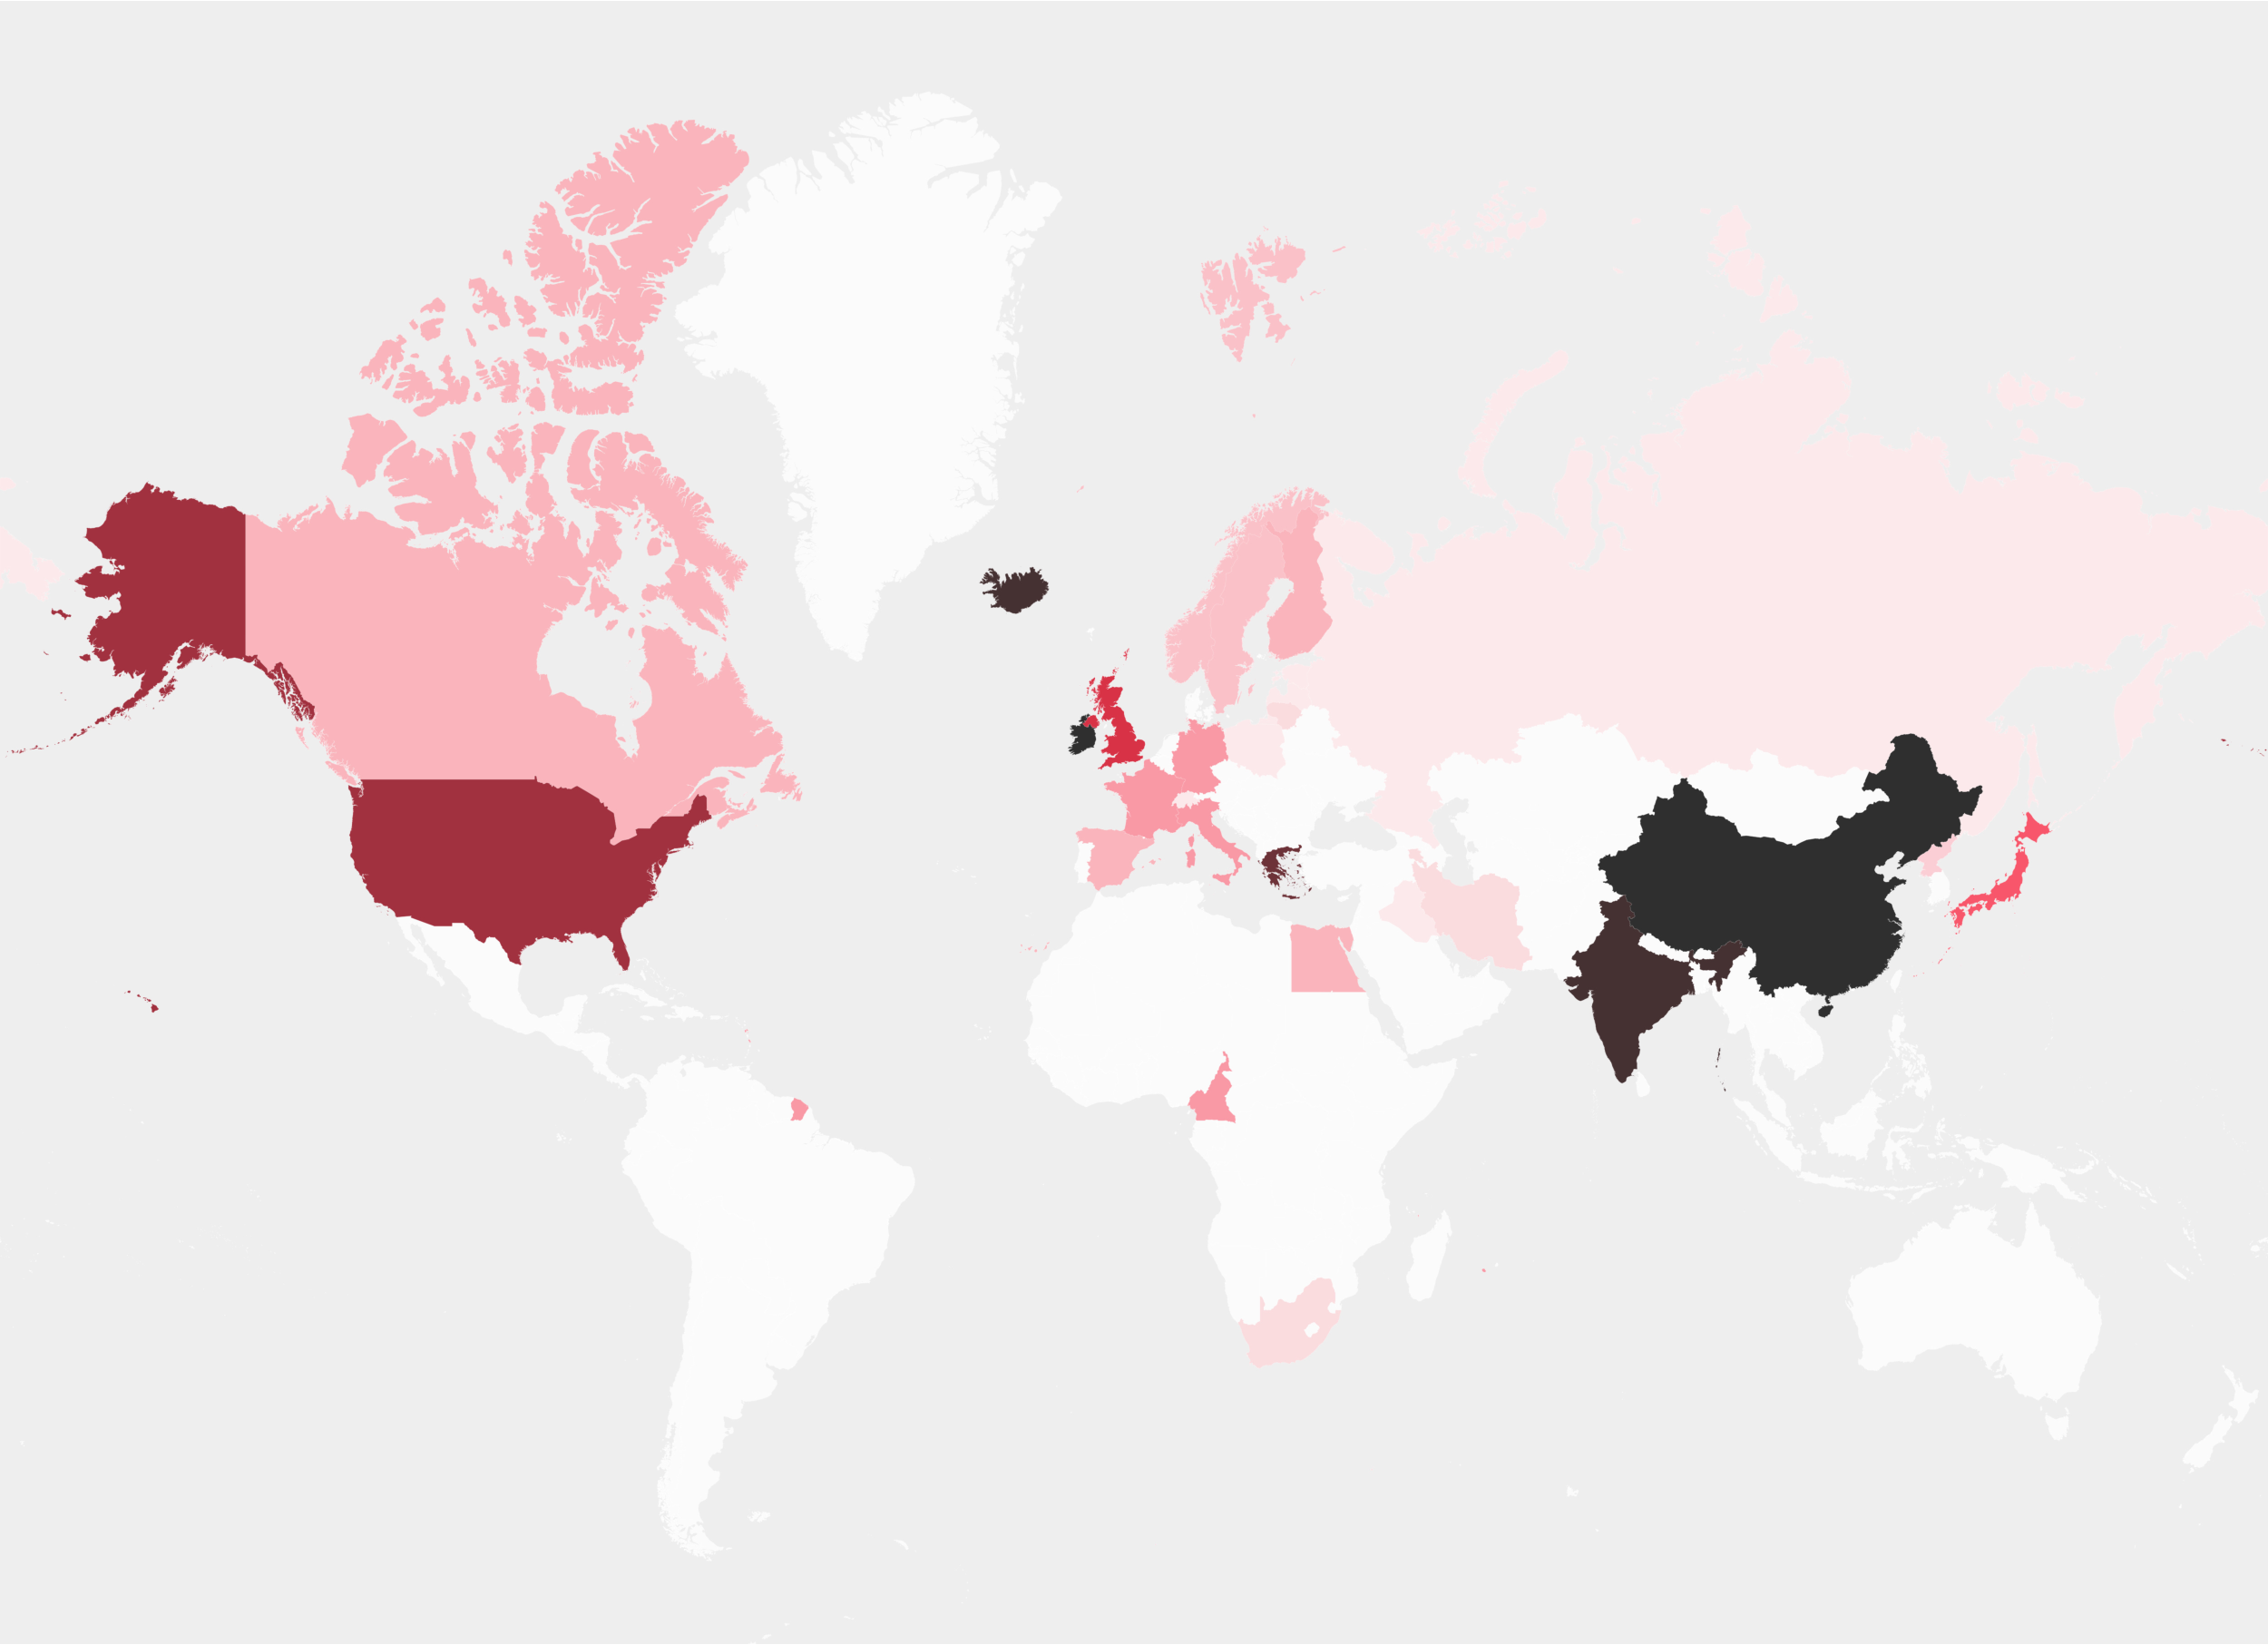
\includegraphics[width=0.7\textwidth]{images/monsters-reduced.pdf}
\caption{Geographical distribution of motifs in Thompson's \emph{Motif-Index of Folk Literature} containing the WordNet concept `monster'. The color gradient (from black via white to red) represents the the frequency of monsters motifs in a country.}
\label{fig:monster-map}
\end{sidewaysfigure}

Thompson intended his TMI to cover motifs from all over the world. Despite the fact that the references only ``give some preliminary guidance in finding examples of the item concerned''\autocite[24]{thompson:1955}, leading to some notable geographical preferences (India) and geographical gaps (e.g.\ the Arab world)\autocite[see for commentary and resolution][]{el-shamy:1980,el-shamy:1995}, it can be argued that Thompson achieved his goal quite well. The TMI mentions over five hundred different locations ranging from small villages in California to islands around the Coral Sea. This information is unique and can provide us with interesting suggestions about the geographical preferences of certain motifs. Here, I am interested in the geographical distribution of the monsters found in the previous paragraph. Which nations prefer werewolves and where do all those dragons hide out?

For each of the 352 motifs mentioning a monster (according to the classification by WordNet), I extracted all the locations in the references field. The locations were aggregated by country; that is, place names, provinces, and so forth were replaced by the name of their corresponding countries. The geographical distribution is visualized in Figure \ref{fig:monster-map}. The color gradient represents the frequency with which monsters are found in a particular country, ranging from white (zero monsters) to black (most monsters). We can observe a strong preference for sources containing monsters from Ireland, Iceland, India, and, most notably, China. It should be acknowledged that given Thompson's relatively unbalanced data collection, the significance of these findings may be relatively trivial and incomplete, but the results serve as an illustration of the ease with which similar information could be extracted from the TMI and hint at certain trends that could be investigated more thoroughly.

\subsubsection{Black, White, and Red: Color Term Appearance in the TMI}

Color naming has long been of interest to researchers in such diverse fields as psychology, linguistics, and anthropology. It gained renewed interest with the publication of Brent Berlin and Paul Kay's groundbreaking study \emph{Basic Color Terms: Their Universality and Evolution}.\autocite{berlin:1969} Their main hypothesis was that ``color categorization is not random and the foci of basic color terms are similar in all languages''\autocite[10]{berlin:1969}. This universalist hypothesis, which states that the addition of colors to a language follows a more or less implicational hierarchy (all languages distinguish the concepts \emph{black} and \emph{white}, languages with three colors add \emph{red} to their arsenal, but no language has only \emph{red} and \emph{white}), has withstood the test of time in key respects, despite the vast amount of critique from more culture-relativistic oriented researchers.

The discoveries of Berlin and Kay also gave impetus to folklore studies. \citeauthor{bolton:1979}, for example, demonstrated that there is a positive correlation between the relative salience of color categories in folktales and the evolutionary development as proposed by Berlin and Kay\autocite{bolton:1979}. In other words: the higher the color in the hierarchy, the more frequently it occurred in folktales. In a recent study, \citeauthor{hemming:2012} proposes an evolutionary source underlying the resonance of the tricolor in symbolic contexts all over the world.\autocite{hemming:2012}

It is to be expected that the importance of color terms will find its reflection in the TMI as well. An example of a motif containing a color name is the motif Z65.1.1 \emph{Red as blood, white as snow, (and black as raven)}, which in Western folklore is most closely associated with the tale of ``Snow White'' (classified as ATU 709 in Uther 2004). This motif neatly reflects the importance of the tricolor \emph{black}, \emph{white}, and \emph{red}. To (tentatively) investigate whether the TMI as a whole reflects the hierarchy of color terms as proposed by Berlin and Kay, MOMFER was used to search for all motifs that mention a color name using the field-specific search query \texttt{wn:color}. This results in 581 motifs containing either chromatic (i.e.\ blue, green, etc.) or achromatic (i.e. black, white, and gray) colors. Figure \ref{fig:color-terms} visualizes the distribution of the color terms in these motifs. The size of the plates represents the frequency with which each color occurs in the TMI. The clear significance of the tricolor black, white, and red is in accordance with findings in previous studies. Again, it must be noted that the current investigation serves only to illustrate how MOMFER can serve as a tool to extract (new) information from TMI. However, it is noteworthy that even in a limited corpus such as the TMI the three colors \emph{black}, \emph{white}, and \emph{red} are indeed the most common.

\begin{figure}
    \centering
    
\includegraphics[width=\textwidth]{images/color-terms.pdf}
    \caption{Visualization of color terms in the \emph{Motif-Index of Folk Literature}. Plates are sized according to the frequency of their corresponding color.}
    \label{fig:color-terms}
\end{figure}

\subsubsection{Marvelous Men, Deceptive Women}

Thompson's TMI has been subjected to a number of gender studies. Torborg Lundell in particular points to a range of gender biases present in the index and makes a strong case for some textual revisions to it\autocites{lundell:1983,lundell:1989}[for a different view, see][83--85]{el-shamy:1990}:
\begin{quote}
    The Motif-Index in general (1) overlooks gender identity in its labelling of motifs, thus lumping male and female actions or characters under the same, male-identified heading or (2) disregards female activity or (3) focuses on male activity at the cost of female.\autocite[150]{lundell:1989}
\end{quote}
Leaving any intrinsic commentary aside, I decided to investigate quantitatively how prominent these gender biases are. I extracted all motifs from the TMI mentioning either a female character or a male character. In this example, the advantage of the semantic word expansion of MOMFER becomes apparent. In the previous case study it would be possible manually to extract all motifs containing a color term (although this would be quite a time-consuming exercise), because the list of possible primary colors is finite and quite small. Extracting all mentions of male and female characters, however, is barely possible by hand, because of the endless list of partial synonyms in both categories (e.g.\ lumberjack, carpenter, etc.). All these words are captured by the semantic expansion mechanism of MOMFER, however, yielding the wanted results.

\begin{figure}[t]
    \centering
    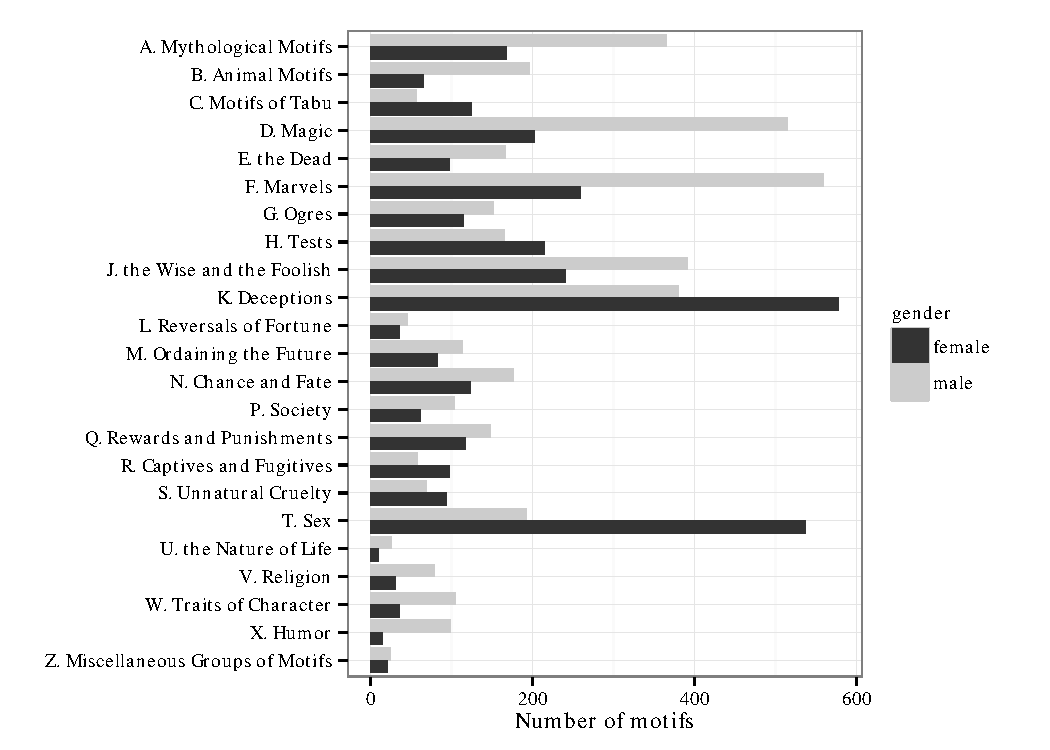
\includegraphics[width=\textwidth]{images/tmi-gender.pdf}
    \caption{Distribution of male versus female entities in \emph{Thompson's Motif-Index of Folk Literature}.}
    \label{fig:tmi-gender}
\end{figure}

I issued two queries: \texttt{wn:male} and \texttt{wn:female}, resulting in 4,178 motifs containing a male character and 3,318 motifs mentioning a female character. These numbers may already indicate some gender biases, since there is no a priori reason to assume that men are more common in stories than women. The gender biases become even more prominent when we look at the distribution of male versus female characters over the main categories in the TMI. Figure \ref{fig:tmi-gender} shows that male characters dominate most motif categories. They are most prominent in \emph{Mythological Motifs} (Category A), \emph{Magic} (Category D), \emph{Marvels} (Category F), and the \emph{Wise and the Foolish} (Category J). Women, on the other hand, dominate the categories \emph{Deception} (Category K) and \emph{Sex} (Category T). These results confirm previous investigations and amplify the need for caution for modern scholars when exploring motifs mentioning male and female personas in the index.

\section{Motif Classification}\label{sec:motif-classification}

While the motif search engine MOMFER allows researchers to more efficiently access the TMI in order to find the motifs that belong to a particular folktale, it remains somewhat problematic that manually assigning motifs to large-scale collections of folktales is a time-consuming, error-prone, and laborious activity. In recent years, a number of new folktale digitization initiatives have been undertaken on a scale that demands for the development of new ways to enrich these collections at different facets such as motifs.\autocite{abello:2012,barre:2012,meder:2010,meder:2016} The remainder of this chapter is devoted to the development of a computational system to automatically identify motifs in folktales, which can be employed to large-scale collections of folktales. Besides reducing manual labor, such a system is relevant for a number of reasons. First, it allows researchers to investigate how folktales have changed through time in terms of their motif material. It is only since the appearance of the Brothers Grimm's version of ``Little Red Riding Hood'', for example, that the girl and her grandmother are rescued from the wolf's belly (cf.\ Chapter \ref{chp:red-riding-hood}). Extracting motifs from texts also allows researchers to find new relationships between folktales, which could tell us more about their evolutionary lineages and origins. 

Only a handful of studies have explored computational systems for motif identification. \citeauthor{voigt:1999} for example, have shown that it is possible to automate motif identification in folklore text corpora by automatically grouping texts based on their content similarities.\autocite{voigt:1999} According to \citeauthor{voigt:1999}, the presence of common motifs can be derived from co-occurrences of keywords in the texts. For folklore researchers, however, such results are not easily interpretable, as these derived motifs are merely represented as principal components to which no recognizable label -- such as a motif from the TMI -- is assigned. To more directly accommodate folktale researchers' practice of assigning motifs from the TMI to folktales, Antal van den Bosch and I have explored and compared two computational systems on the task of automatically identifying motifs in folktales.\autocite{karsdorp:2013} We have shown that a relatively simple model that is often used in information retrieval contexts is able to confidently identify motifs in a large number of folktales. 

Both computational systems presented by \citeauthor{karsdorp:2013} make the naive assumption that the occurrence of a motif is independent of the occurrence of other motifs. It can be argued, however, that occurrences of motifs in a folktale are -- at least partially -- mutually predictive. This suggests that we can achieve better performance by taking into account the dependencies between motifs. My aim in this chapter is to further explore and build on these previous models of motif identification while thoroughly investigating and comparing a number of approaches that do incorporate the dependencies between motifs. 

In what follows, I will first describe the data resources and data annotations used to construct this system (Section \ref{sec:classification-data}). Subsequently, I will provide a detailed description in Section \ref{sec:multi-label-classification} of the multi-label classification problem and a number of problem transformation techniques that allow us to more efficiently address this problem. Finally, after having discussed the experimental setup in Section \ref{sec:classification-setup}, I will present the empirical results in Section \ref{sec:motif-classification-results}.


\subsection{Data and Annotation}\label{sec:classification-data}

Crucially, the construction of an automated classification system requires a large data set of stories that are annotated with motifs. Since no such annotated collection of stories is available, the first step in constructing the system consists in compiling a sufficiently large corpus with motif annotations. In the present study, I have opted to compile this corpus based on a set of folktales from the Dutch Folktale Database\autocite{meder:2010}, as most of the folktales in the Dutch Folktale Database have been manually linked to the types in \citeauthor{uther:2004}'s tale type catalog (as far as it was possible to establish \emph{any} such link). These links between particular instances of tales and corresponding tale types provide us with a set of primary descriptive motifs that constitutes a folktale type, and, by definition in its instantiations. Each tale type in \citeauthor{uther:2004}'s tale type catalog provides a short summary of the most common plot developments along with a sequence of motifs from the TMI. An example of such a tale type description reads as follows: 
\begin{quote}
ATU 327A, \textbf{Hansel and Gretel.} A (poor) father (persuaded by the stepmother) abandons his children (a boy and a girl) in the forest [S321, S143]. Twice the children find their way back home, following scattered pebbles [R135]. On the third night, birds eat the scattered peas (bread-crumbs) [R135.1]. The children come upon a gingerbread house which belongs to a witch (ogress) [G401, F771.1.10, G412.1]. She takes them into her house. The boy is fattened [G82], while the girl must do house-work. The witch asks the boy to show his finger in order to test how fat he is [G82.1], but he shows her a bone(stick) [G82.1.1]. When the witch wants to cook the boy, the sister deceives her by feigning ignorance and pushes her into the oven [G526, G512.3.2]. [\ldots] The children escape, carrying the witch's treasure with them.  Birds and beasts(angels) help them across water. They return home.
\end{quote}
This example shows that the tale type ATU 327A contains twelve motifs, such as S321 \emph{Destitute parents abandon children}, G401 \emph{Children wander into ogre's house}, G82.1 \emph{Cannibal cuts captive's finger to test fatness} and G526 \emph{Ogre deceived by feigned ignorance of hero}. 

\begin{figure}
  \centering
  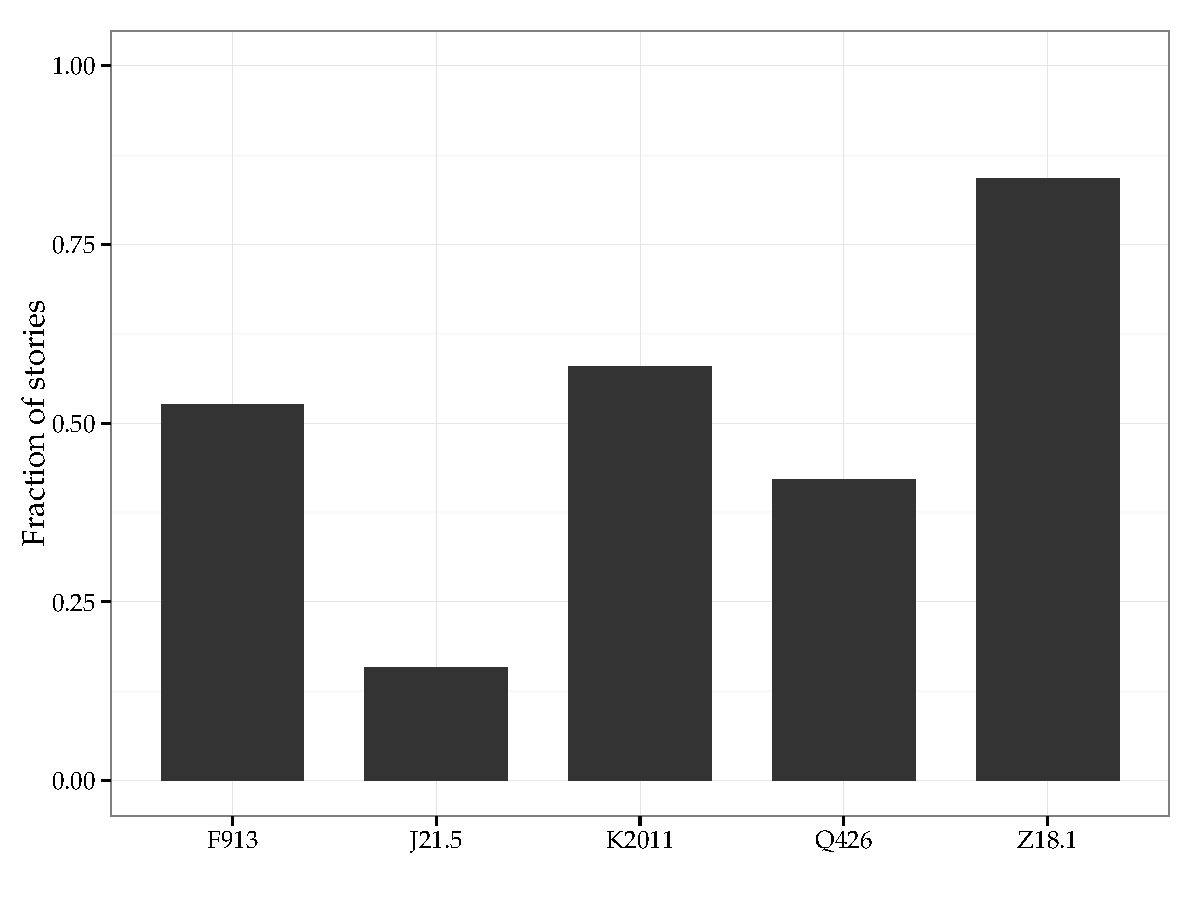
\includegraphics[width=\textwidth]{images/atu-333-motifs.pdf}
  \caption{Distribution of motifs from tale type ATU 333 ``Little Red Riding Hood''. On the basis of 19 instances of tale type ATU 333, the plot displays the fraction of instances in which one of the tale type motifs occurs.}
  \label{fig:atu-333-motifs}
\end{figure}

However, particular instances of a tale type do not necessarily contain all motifs listed under their corresponding tale type; they rather comprise a subset of the relevant motifs. Thus, the corpus compilation requires a second step, in which the tale type motifs that were assigned to a particular instance of the type that did not exhibit them were removed. To give an example of this `filtering' step, in Figure \ref{fig:atu-333-motifs} I show the distribution of the motifs of tale type ATU 333 ``Little Red Riding Hood'' for 19 instances in the Dutch Folktale Database. While the tale type ATU 333 enumerates a set of five primary motifs\footnote{I.e., J21.5 \emph{Do not leave the highway.}, Z18.1 \emph{What makes your ears so big?}, K2011 \emph{Wolf poses as ``grandmother'' and kills child.}, F913 \emph{Victims rescued from swallower's belly.}, and Q426 \emph{Wolf cut open and filled with stones as punishment.}}, most instances of the type exhibit only a subset of these motifs. In fact, the distribution shows that none of Red Riding Hood's tale type motifs mentioned by \citeauthor{uther:2004} is present throughout all instances of the tale type.\autocite{uther:2004}

In total, the complete corpus consists of 1,427 annotated stories. The stories were tokenized using the tokenizer Ucto, which was configured for the Dutch language.\footnote{Available from \url{https://languagemachines.github.io/ucto/}.} The tokenized corpus contains 790,990 word forms (excluding punctuation) and 42,623 word types. On average, each story is about 554 words long ($\sigma=742.9$). The 1,427 stories exhibit 398 different tale types from \citeauthor{uther:2004}'s tale type catalog. The collection contains 2,483 motif annotations, which amounts to about two motifs per story on average ($\sigma=1.46$). The number of unique motifs in the collection equals 747.

\subsection{Multi-label Ranking}\label{sec:multi-label-classification}

In this section, I present a detailed formal description of the motif identification task. Let $d$ denote a story and $C$ the corpus of annotated stories. Each story $d_i$ is labeled with a subset of motifs $M_i \subset M$, with $M$ denoting the set of unique motifs in $C$ (i.e.\ $|M|=747$). In the approach presented here, the motif identification task is framed as a ranking problem. This means that I tackle this task by computing a ranking of all unique motifs for each story. In computing this ranking, I aim to allocate the highest positions in these rankings to the most relevant motifs. The reason for approaching the task as a ranking problem rather than a classification problem is the following: because a particular story's annotated motif subset $M_i$ can only consist of motifs that are listed under the story's corresponding tale type, the subset $M_i$ does not necessarily contain all motifs that are potentially relevant for its characterization. It is possible that motifs listed under \emph{different} tale types also prove to be relevant even though they are not part of a story's primary descriptive units. The benefit of a ranking approach is that, instead of yielding a single output (as would be the case with classification), it provides a list of motifs ordered by relevance in which the highest ranks are allocated to the most relevant motifs. Thus, by taking a ranking approach I do not \emph{impose} a classification on a story, but rather, I provide a `motif recommendation list' from which scholars can select the motifs that apply.

Let us now turn to the formal description of the motif identification task, which is framed as a multi-label ranking problem. Let $D$ represent the training data consisting of $N$ annotated stories. Each story $d_i$ is associated with a feature vector $\vec{\mathbf{x_i}}$ and a motif subset $M_i \subset M$, i.e.\ $d_i = (\vec{\mathbf{x_i}}, M_i)$. To illustrate this representation, consider the following four versions of ATU 333 ``Little Red Riding Hood'':

\begin{table}[h]
\centering
\begin{tabular}{l|l|l}
\toprule
$d_1$ & $\vec{\mathbf{x_1}} = (x_1, x_2, \ldots, x_V)$ & $M_1 = \{ \text{F913, Q426}\}$ \\
$d_2$ & $\vec{\mathbf{x_2}} = (x_1, x_2, \ldots, x_V)$ & $M_2 = \{ \text{F913, Z18.1}\}$ \\
$d_3$ & $\vec{\mathbf{x_3}} = (x_1, x_2, \ldots, x_V)$ & $M_3 = \{ \text{K2011, Z18.1}\}$ \\
$d_4$ & $\vec{\mathbf{x_4}} = (x_1, x_2, \ldots, x_V)$ & $M_4 = \{ \text{F913, Q426}\}$ \\
\bottomrule
\end{tabular}
\end{table}

\noindent Given this representation, the task of the multi-label ranking algorithm is to learn a ranking function $f$, which takes as input a story $d$ for which the motifs are unknown, i.e.\ $d = (\vec{\mathbf{x}}, ?)$, and produces a ranking $R$ which consists of all motifs $M$ ordered by their relevance to $d$, i.e.\ $f(d) \rightarrow R$. In what follows, I will discuss and compare the benefits and downsides of two existing multi-label ranking methods, i.e. `Binary Relevance Transformation', and `Label Power Set Transformation'. Subsequently, I will suggest a new multi-label ranking method, which I will call `Tale Type Transformation'. Each of these ranking methods is a `problem transformation method'\autocite{tsoumakas:2007,tsoumakas:2010}. The goal of these methods is to transform the data in such a way that we can employ single-label learning algorithms, which are computationally more efficient and easier to apply than multi-label ones.

\paragraph{PT-1: Binary Relevance Transformation}

The `Binary Relevance' method decomposes the multi-label ranking problem into $|M|$ \emph{binary} ranking problems. The method consists of the following steps: first, for each motif $m \in M$ a new data set $D_i$ is constructed in which each document $d_i$ is associated with a binary label $y_i \in \{0, 1\}$. $y_i$ takes as value $1$ if motif $m_i$ is present in document $d_i$, and $0$ if otherwise. This transformation process can be illustrated by applying it to the example data presented above, which results in the following four data sets:

\begin{table}[h]
\centering
\begin{tabular}{lr}
\multicolumn{2}{c}{$D_1$} \\
\toprule
$d_1$ & $\text{F913}$\\
$d_2$ & $\neg{\text{F913}}$\\
$d_3$ & $\text{F913}$\\
$d_4$ & $\text{F913}$\\
\bottomrule
\end{tabular}
\quad
\begin{tabular}{lr}
\multicolumn{2}{c}{$D_2$} \\
\toprule
$d_1$ & $\text{Q426}$ \\
$d_2$ & $\neg{\text{Q426}}$ \\
$d_3$ & $\neg{\text{Q426}}$ \\
$d_4$ & $\text{Q426}$ \\
\bottomrule
\end{tabular}
\quad
\begin{tabular}{lr}
\multicolumn{2}{c}{$D_3$} \\
\toprule
$d_1$ & $\neg{\text{K2011}}$\\
$d_2$ & $\neg{\text{K2011}}$\\
$d_3$ & $\text{K2011}$\\
$d_4$ & $\neg{\text{K2011}}$\\
\bottomrule
\end{tabular}
\quad
\begin{tabular}{lr}
\multicolumn{2}{c}{$D_4$} \\
\toprule
$d_1$ & $\neg{\text{Z18.1}}$ \\
$d_2$ & $\text{Z18.1}$ \\
$d_3$ & $\text{Z18.1}$ \\
$d_4$ & $\neg{\text{Z18.1}}$ \\
\bottomrule
\end{tabular}
\end{table}

The second step consists in training a ranking function $f$ for each of these transformed data sets and applying these binary ranking functions to a new input story. Each ranking function $f_{m_i}$ generates a score (for instance, in the case of a probabilistic ranking function, between 0 and 1) which expresses the confidence that motif $m_i$ is present in one of the stories under consideration. To obtain a final ranking of all motifs, the last step involves aggregating the results of the binary ranking functions into a single list, which is sorted in descending order according to the confidence scores assigned to each motif.

The complexity of the Binary Relevance method scales linearly with the number of unique motifs $|M|$. The clearest advantage of the method, therefore, is its low computational complexity. However, this low complexity comes with a cost; the method is blind to any potential relationships between motifs, or, in other words, it treats all motif occurrences as being independent of each other. 

\paragraph{PT-2: Label Power Set Transformation}

The second problem transformation method turns the multi-label ranking problem into a multi-class ranking problem by transforming each unique motif subset $M_i \in M$ into a distinct class. The following two tables illustrate this transformation process. The table on the left corresponds to the original training data $D$ and the table on the right represents the transformed data set $D'$.

\begin{table}[h]
\centering
\begin{tabular}{ll}
\multicolumn{2}{c}{$D$} \\
\toprule
$d_1$ & $M_1 = \{ \text{F913, Q426}\}$ \\
$d_2$ & $M_2 = \{ \text{F913, Z18.1}\}$ \\
$d_3$ & $M_3 = \{ \text{K2011, Z18.1}\}$ \\
$d_4$ & $M_4 = \{ \text{F913, Q426}\}$ \\
\bottomrule
\end{tabular}
\quad$\rightarrow$\quad
\begin{tabular}{ll}
\multicolumn{2}{c}{$D'$} \\
\toprule
$d_1$ & $A = (\text{F913} \land \text{Q426})$ \\
$d_2$ & $B = (\text{F913} \land \text{Z18.1})$ \\
$d_3$ & $C = (\text{K2011} \land \text{Z18.1})$ \\
$d_4$ & $A = (\text{F913} \land \text{Q426})$ \\
\bottomrule
\end{tabular}
\end{table}

\noindent In this small example set, the Label Power Set method reduces the number of labels for which a prediction has to be made: the original label set consists of four distinct motifs (i.e.\ F913, Q426, Z18.1, K2011), whereas the transformed label set only consist of three distinct classes (i.e.\ A, B and C). Because the Label Power Set method considers each unique motif subset to be a distinct class label, it implicitly models dependencies between labels. It should be noted, however, that with large label sets the Label Power Set method often yields an (exponential) increase (rather than a decrease) of the number of labels. Moreover, most labels in the transformed data set are associated with only a few stories. This label sparsity is one of the main drawbacks of the Label Power Set method, because it is difficult to build effective learning algorithms on the basis of a small number of examples.

\paragraph{PT-3: Tale Type Transformation}

In order to counter the drawbacks of the aforesaid transformation methods, I present a new problem transformation method. This method is related to the Label Power Set method, but it does not suffer from the aforementioned label sparsity problem to the same extent. In Section \ref{sec:classification-data}, it was pointed out that each story in the annotated corpus is labeled with a tale type from \citeauthor{uther:2004}'s tale type catalog, and that each tale type is associated with a set of distinctive motifs. To tackle the multi-label ranking problem, the problem transformation method I propose aims to exploit the information about tale types by means of a two-tier method. This two-tier method involves the following subsequent steps: first, the original training data $D$ is transformed to a new data set $D'$ in which each story $d_i$ is associated with a single label $y_i$, which corresponds to the tale type $t \in T$ of $d_i$, where $T$ refers to the complete set of tale types in the training data $D$. To illustrate this transformation process, consider the tables below.

\begin{table}[h]
\centering
\begin{tabular}{ll}
\multicolumn{2}{c}{$D$}\\
\toprule
$d_1$ & $\{\text{K335.1.4, K1161, N776}\}$ \\
$d_2$ & $\{\text{L161, F96}\}$ \\
$d_3$ & $\{\text{K1161}\}$ \\
$d_4$ & $\{\text{A2741.1, F1025.1}\}$ \\
\bottomrule
\end{tabular}
\quad$\rightarrow$\quad
\begin{tabular}{ll}
\multicolumn{2}{c}{$D'$}\\
\toprule
$d_1$ & $y_1 = \text{ATU\ 0130}$ \\
$d_2$ & $y_2 = \text{ATU\ 0301}$ \\
$d_3$ & $y_3 = \text{ATU\ 0130}$ \\
$d_4$ & $y_4 = \text{ATU\ 0295}$ \\
\bottomrule
\end{tabular}
\end{table}

The second step consists in training a multi-class ranking function for this transformed data set. When a new, unseen story $d$ is presented, the algorithm generates a score for each tale type $t \in T$ which stands for the confidence that the tale type of story $d$ equals $t$. In the case of a probabilistic ranking function, this score represents the probability $p(t|d)$ that story $d$ belongs to tale type $t$. To arrive at a final ranking of all motifs in $M$, we can employ this tale type probability to assign the probability $p(t|d)$ to each of the motifs associated with $t$. However, this would result in a relatively uninformed ranking, as all motifs that belong to a particular tale type would be scored equally. As such, there would be no way to determine which motif is to be preferred over another. To obtain a more fine-grained ranking, I propose to compute the joint probability of a tale type given a story (i.e.\ $p(t|d)$) and the prior probability $p(m|t)$ of a motif given a tale type, i.e.\ $p(t|d) \times p(m|t)$. Subsequently, we can rank the motifs according to this product. The prior probability can be computed on the basis of the frequencies of a motif's occurrence with a particular tale type in the training data $D'$. 

\subsection{Experimental Setup}\label{sec:classification-setup}

\paragraph{Models}

Each of the three problem transformation methods requires a base classifier. In this study, I opted for a Maximum Entropy classifier (also known as a Logistic Regression classifier). I used the probabilistic decision function of this classifier to produce the required rankings, and I employed Scikit-Learn's implementation of this classifier with L2 regularization. In all experiments, the regularization strength parameter $C$ was set to 500.\autocite{sklearn:2011}

\paragraph{Features}

While other, more sophisticated features can be easily adopted, the present approach depends on simple `bag-of-words' features, which have proven to be highly efficient in numerous computational approaches to textual data. Given a corpus $C$ consisting of a vocabulary $V$ (i.e.\ all unique words in the corpus), bag-of-words models represent documents as histograms over the vocabulary, or, in other words, as vectors consisting of frequencies for each unique word. Given a story $d$, the vector representation $\vec{\mathbf{w}}^{(d)}$ is $(w_1, w_2, \ldots, w_{|V|})$, where $w_i$ represents the number of occurrences of word $i$ in story $d$. In addition to these bag-of-words features, I make use of so-called `character $n$-gram features', which represent counts of substrings of words. By setting $n$ to four, for example, a word such as \emph{wizard} is represented by the following substrings: \texttt{wiza}, \texttt{izar}, and \texttt{zard}. On the basis of these substrings, a new vector representation is created which represents a histogram over all unique substrings $s \in S$, i.e.\ $\vec{\mathbf{s}}^{(d)} = (s_1, s_2, \ldots, s_{|S|})$, where $s_i$ represents the number of times the substring $i$ occurs in story $d$.

It is common practice in many computational applications to weigh these frequency vectors for feature importance. As such, I transformed the frequency vectors by means of Parsimonious Language Models as proposed by \citeauthor{hiemstra:2004}.\autocite{hiemstra:2004} Parsimonious Language Models represent a probabilistic alternative to traditional tf-idf weighting schemes\autocite{manning:2008}, and have proven to be highly efficient in Information Retrieval. For each document $d$, a parsimonious language model is defined as:
\begin{equation}
P(t_1,\ldots,t_n|d) = \prod^n_{i=1} (1 - \lambda) P(t_i|D) + \lambda P(t_i|d)
\end{equation}
where $D$ represents the complete training collection, and $t$ represents either a word or a character $n$-gram feature. The estimate of $P(t|d)$ is maximized using an Expectation-Maximization algorithm (cf.\ Algorithm \ref{alg:expectation-maximization}). The hyperparameter $\lambda$ controls the spread of probability mass to features, i.e.\ how much weight is assigned to each feature. With $\lambda < 1$, the probability mass is moved to fewer features than a maximum likelihood estimate of the documents would, and the probability mass moves to even fewer features as $\lambda$ approaches 0. This results in a `peaky' distribution of feature weights, with only a few strongly weighted features for each document.

\begin{algorithm}[t]
\For{feature $t_i \in d$}{
    \While{not converged}{
        $e_i = tf(t_i) \cdot \frac{\lambda P(t_i|d)}{(1-\lambda)P(t_i|D) + \lambda P(t_i|d)}$ \;
        $P(t_i|d) = \frac{e_i}{\sum_i e_i}$ \;
        }
}
 \caption{Expectation-Maximization Algorithm}
 \label{alg:expectation-maximization}
\end{algorithm}

\paragraph{Evaluation}

For the evaluation of the models, I used a $n$-fold cross-validation setup. In this setup, all stories are shuffled, and subsequently partitioned into $n$ subsets of equal size. The model is set to run for $n$ iterations. At each iteration a different part or `fold' acts as a test set, and the remaining folds are combined to form the training set. In the experiments below, $n$ is set to 4.

The performance of the models is measured by means of five evaluation metrics, i.e.\ Average Precision, One Error Score, Is Error score, Margin Score, and Ranking Loss. Each of these metrics addresses a different aspect of the performance quality of the models, as they each ask different questions about the rankings:\autocite{tsoumakas:2010}
\begin{description}
\item[Average Precision:] Are most or all of the target motifs high up in the ranking?
\begin{equation}
\text{AP} = \frac{\sum^n_{k=1} (P(k) \times rel(k))}{\text{number of relevant motifs}}
\end{equation}
where $k$ is the position in the ranked list of $n$ retrieved motifs. $P(k)$ represents the precision at $k$ and $rel(k) = 1$ if the item at position $k$ is relevant, $rel(k) = 0$ otherwise. The Average Precision yields a score between 0 and 1, where 1 indicates a perfect ranking.
\item[One Error:] For what fraction of test documents is the highest-ranked motif \emph{incorrect}?
\begin{equation}
\text{One Error} = \frac{1}{n} \sum^n rel(1)
\end{equation}
The One Error Score is a value between 0 and 1, where 0 indicates that for all of the test documents the highest rank motif is correct.
\item[Is Error:] What fraction of rankings is \emph{not} perfect?
\begin{equation}
\text{Is Error} = \frac{1}{n} \sum^n_{d=1} \text{AP}(d) < 1
\end{equation}
The Is Error Score is a value between 0 and 1, where 0 means that in all generated rankings, all relevant motifs are ranked highest. The Is Error Score is complementary to the Average Precision Score, as it represents the fraction of test documents that has an Average Precision score smaller than 1.
\item[Margin:] What is the absolute rank difference between the highest ranked irrelevant motif and the lowest ranked relevant motif averaged across test documents?
\begin{equation}
\text{Margin} = \frac{1}{n} \sum^n |k_{\text{highest irrelevant}} - k_{\text{lowest relevant}}|
\end{equation}
The Margin Score is a value from 0 to $n$, where $n$ is the number of possible motifs in the ranking. The closer to 0, the smaller the absolute difference between relevant motifs, and the better the ranking.
\item[Ranking Loss:] What is the number of times that relevant motifs are ranked lower than irrelevant motifs, first averaged within one document, then across all test documents.
\begin{equation}
\text{L} = \frac{1}{n} \sum^n_{i=1} \frac{1}{|M_i| |\bar{M_i}|} |\{(m_a, m_b): k_a > k_b, (m_a, m_b) \in M_i \times \bar{M_i}\}|,
\end{equation}
where $\bar{M_i}$ is the complementary set of $M_i$.
The Ranking Loss score is equivalent to the complement of the area under the ROC curve.\autocite{rubin:2012} It is a value between 0 and 1, where 0 indicates a perfect ranking.
\end{description}

\subsection{Results}\label{sec:motif-classification-results}

\begin{table}
\centering
\begin{tabular}{lccccc}
\toprule
     & AP   & One Error & Is Error & Ranking Loss & Margin \\ \midrule
PT-1 & .775 & .249      & .348     & .051      & 23.15 \\
PT-2 & .760 & .270      & .371     & .050      & 22.61 \\
PT-3 & \textbf{.801} & \textbf{.243} & \textbf{.323} & \textbf{.021} & \textbf{8.25} \\
\bottomrule
\end{tabular}
\caption{Motif ranking results. The table provides the Average Precision score, One Error score, Is Error score, Ranking Loss and Margin score for all three problem transformation methods, i.e.\ PT-1: Binary-Relevance, PT-2: Label Power Set and PT-3: Tale Type Transformation.}
\label{tab:motif-ranking-results}
\end{table}

Table \ref{tab:motif-ranking-results} presents the results of the experiments. The table provides the Average Precision score, One Error score, Is Error score, Ranking Loss, and Margin score for the three problem transformation methods set out in Section \ref{sec:multi-label-classification}. Observe that PT-3 outperforms the other two transformations methods across all evaluation metrics. Although all models are able to generate motif rankings with relatively high Average Precision (PT-1: $0.78$, PT-2: $0.76$, PT-3: $0.8$), the difference between the margin score of PT-1 (23.15) and PT-2 (22.61), and that of PT-3 (8.25) is sufficiently large to support the hypothesis that incorporating mutual motif relations via tale type dependencies into the model leads to a performance boost. With respect to the `Ranking Loss' and `One Error' score, PT-3 exhibits a small performance increase compared to the other models: PT-3 generates rankings in which the top ranked motif is correct in 76\% of the cases. Finally, the tale type transformation method marginally outperforms the other two transformation methods in producing perfect rankings, with 68\% of its rankings having an Average Precision of 1.0.

In what follows, I will provide a more detailed analysis of the experimental results as well as possible explanations for the performance differences between the models. I hypothesize that the Tale Type Transformation method (PT-3) has two main advantages over the other two transformation methods, which leads to the observed difference in performance. First, PT-3 implicitly models dependencies between motifs by incorporating their overarching tale type, whereas in the Binary Relevance model (PT-1) all predictions happen independently of each other. While the Label Power Set method (PT-2) is also designed to implicitly take some of the dependencies between motifs into account, it suffers from a different problem: PT-2 can lead to severe label sparsity when only a very small number of examples is available for many unique motif subsets. The second advantage of the PT-3 method is that, because of its two-tier architecture, it is less vulnerable to such label sparsity issues. 

\begin{figure}[t]
\centering
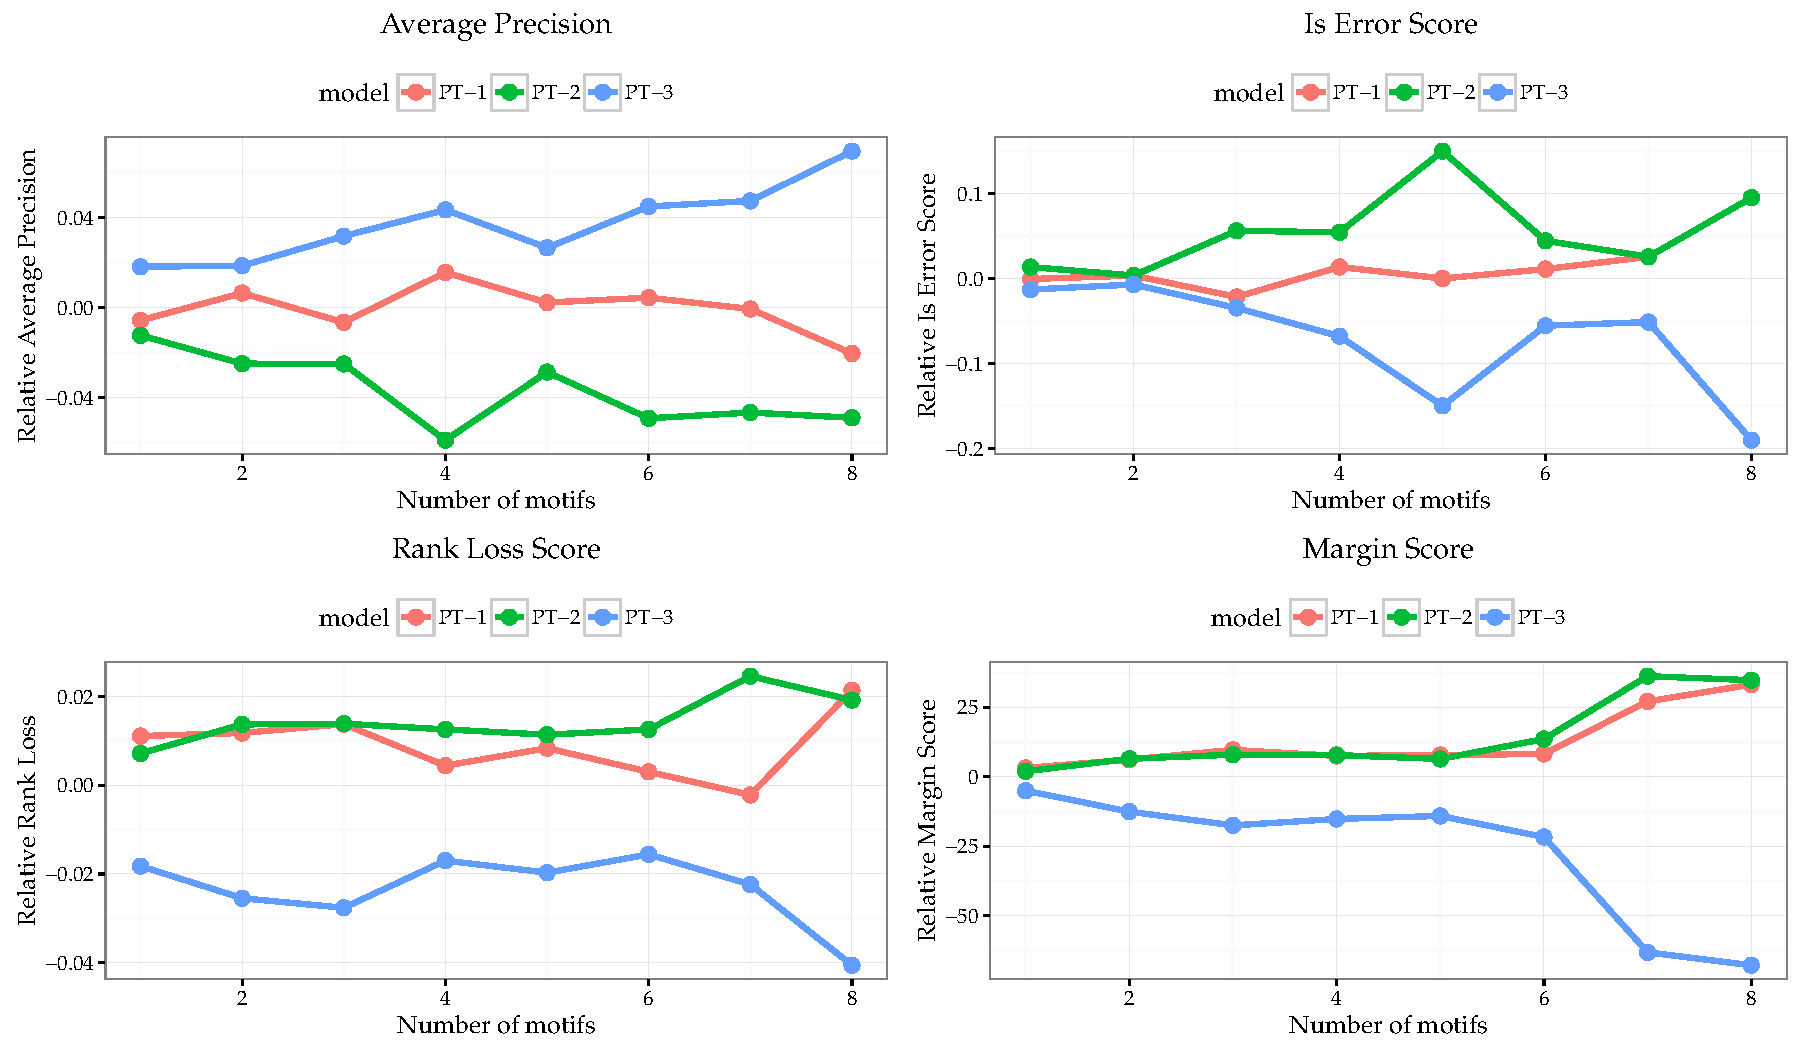
\includegraphics[width=\textwidth]{images/motif-evaluation-scores-size.pdf}
\caption{Interaction between the number of motifs per document and model performance. In order of appearance, the plots show the `Average Precision', `Is Error' score, `Ranking Loss' score and `Margin' score for subsets of test documents grouped on the basis of how many motifs they contain. The One Error score is not included in the plot, as it highly correlates with the Average Precision.}
\label{fig:motif-size-classification}
\end{figure}

If these hypotheses hold, we can expect that models in which motif dependencies are taken into account perform even better on stories with an increasing amount of motifs. To empirically ground this hypothesis, I recompute the evaluation metrics for subsets of test documents which are grouped by the number of motifs they contain. Figure \ref{fig:motif-size-classification} illustrates the \emph{relative} performance differences between the three models for subsets of stories with an increasing number of motifs. Note that the results for this plot have been centered around zero in order to obtain a clearer picture of the differences. The plot shows that, as the number of motifs per document increases, the performance difference between PT-3 on the one hand and PT-1 and PT-2 on the other becomes larger. This effect can be observed for all four given evaluation metrics. 

Note that, contrary to expectations, the Label Power Set method (PT-2) in Figure \ref{fig:motif-size-classification} does not exhibit a performance advantage relative to the more naive Binary Relevance method. In fact, PT-2 consistently performs worse than the other two transformation methods. The main reason why PT-2 lags behind the other methods, I wish to argue, is that it suffers from the aforementioned label sparsity problem: there are not nearly enough examples to build effective classifiers. As the number of unique motifs increases, this sparsity problem becomes more severe because the number of possible motif combinations grows. As such, PT-2 (and also, albeit to a lesser extent, PT-1) exhibits a performance drop on data sets with an increasing number of unique motifs. To this end, it is interesting to compare the performance of the models with respect to the genre distinctions in the tale type catalog by \citeauthor{uther:2004}. This catalog lists over two thousand unique tale types, which are divided into the following seven genres:

\begin{enumerate}
    \item \emph{Anecdotes and Jokes} include classical jokes and riddles. They often end with a punchline and are relatively short;
    \item \emph{Animal Tales} are tales in which the protagonist is usually an animal. They are relatively short and contain one or two prominent motifs;
    \item \emph{Formula Tales} deal with tales in which ``form is all-important''\autocite[229]{thompson:1977}. The tales are often rather short, contain repetition and a small number of motifs;
     \item \emph{Tales of Magic} are spatio-temporally unbound stories. The plot often centers around one protagonist who faces a range of challenges in his or her quest towards some desired object. Tales of Magic can be quite detailed and long both in words and in number of motifs;
    \item  \emph{Realistic Tales} likewise describe adventures and heroes, but in Realistic Tales there is an absence of any form of magic;
    \item \emph{Religious Tales} are comparable to legends. They are spatio-temporally bound stories that occur in the recent past that describe supernatural events and center around religious values;
    \item \emph{Tales of the Stupid Ogre} resemble humorous tales about ogres, devils etc.\ with wondrous aspects.
\end{enumerate}

\begin{figure}[t]
\centering
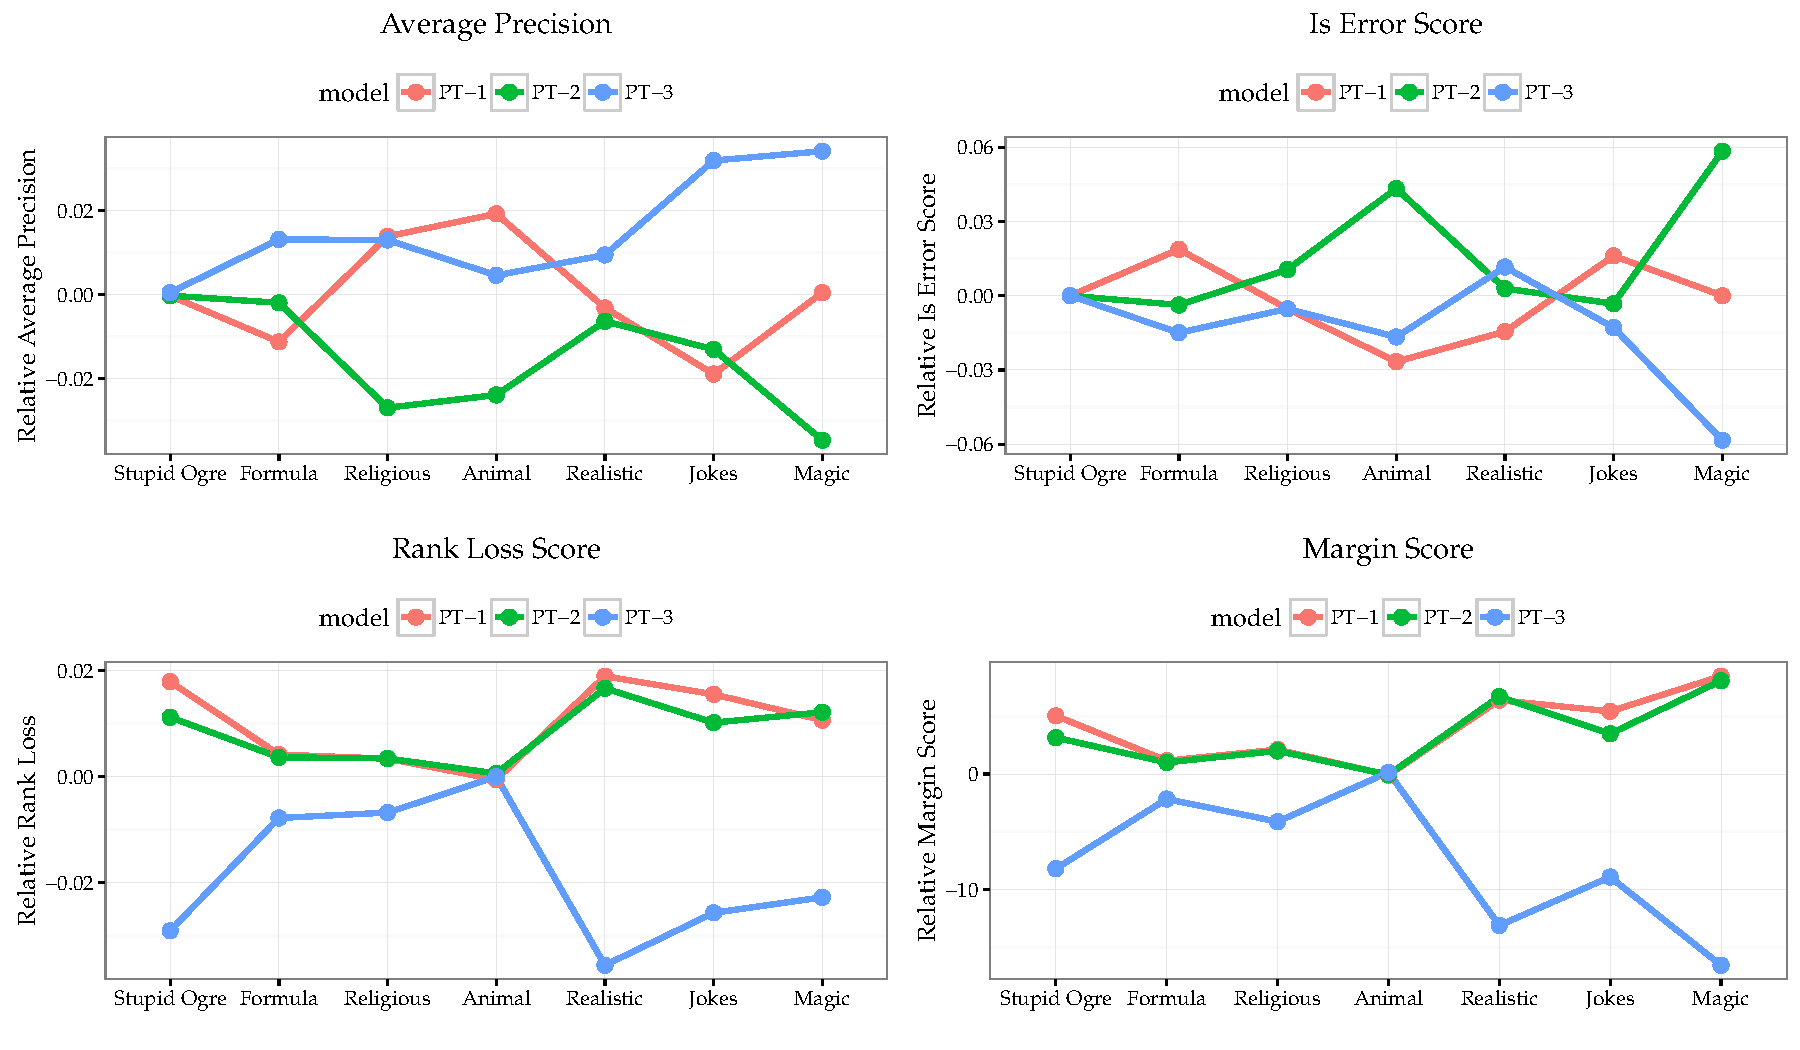
\includegraphics[width=\textwidth]{images/motif-evaluation-scores.pdf}
\caption{Interaction between number of unique motifs per folktale genre and model performance. In order of appearance, the plots show the `Average Precision', `Is Error' score, `Ranking Loss' score and `Margin' score for each folktale genre in \citeauthor{uther:2004}'s tale type catalog. The genres are ordered according to the number of unique motifs they contain.}
\label{fig:motif-classification-genre}
\end{figure}

Figure \ref{fig:motif-classification-genre} illustrates the \emph{relative} performance between the three models for each of these seven genres. The genres have been ordered according to the number of unique motifs they contain. The plots add visual evidence to the hypothesis that there is an interaction between the performance of the models and the number of unique motifs in a genre. Both the `Binary Relevance' and the `Label Power Set' method undergo a performance drop as the number of unique motifs increases. Such a drop is not observed with the `Tale Type Transformation' method, which can be explained by the fact that the number of possible labels in the first tier of PT-3 is much lower than that of the other two transformation methods. Furthermore, it appears that PT-2 suffers the most if the number of unique motifs increases, which can again be attributed to its label sparsity problem.

\section{Conclusion}

In the first part of this chapter, I presented MOMFER, which is a new and fast research tool designed to accompany Thompson's TMI. I set out the production process, documented the query system, and showed how the tool offers new ways to explore the index in three small case studies. A complete collection of all motif indices would be an amazing research tool. MOMFER is a first step towards such an index: with its flat architecture, it enables the inclusion of other motif indices. As Heda Jason notes, proposals for new motifs should be made ``only after it has been found that no other motif index has listed the specific content element in question''\autocite[61]{jason:2000}. An integrated tool such as MOMFER could serve as a warrant for such requirements. The tool serves as a starting point for inviting researchers to join in disclosing other indices so that, more than fifty years after the publication of Thompson's great index, we may finally have a complete index of all folklore motifs.

In the second part of this chapter, I developed a computational system for motif identification in folktales. This system, presented in Section \ref{sec:motif-classification}, frames this identification task as a ranking problem. The goal of such a system is to produce a ranking of motifs for a particular story in which the top ranked motifs represent the most relevant motifs for that particular story. An in-depth comparison of three problem transformation methods (i.e.\ `Binary Relevance' (PT-1), `Power Label Set' (PT-2) and `Tale Type Transformation' (PT-3)) showed that the Tale Type Transformation method (PT-3) can achieve better performance than models that assume that motifs are not mutually predictive (PT-1), because it incorporates dependency relations between motifs through their overarching tale type. Furthermore, it was shown that this model suffers less from the well-known label sparsity problem than existing problem transformation methods such as the Label Power Set method (PT-2). The Tale Type Transformation method is able to quite accurately identify motifs in folktales at an Average Precision of 0.8 on unseen documents.

Because the present study adopts a ranking approach rather than a classification approach, it comes with a great benefit for folklore scholars: the approach presented above does not \emph{impose} a particular all-or-nothing classification on a story, but rather, it provides scholars with \emph{recommendations} about which motifs are likely to be applicable to a story. The combination of this recommendation system with the motif search engine MOMFER can greatly facilitate folklore scholars in their future endeavors to analyze large-scale folktale collections and the relations between folktales and their motifs.

